\documentclass[12pt,a4paper,openright,twoside]{book}
\usepackage[utf8]{inputenc}
\usepackage{disi-thesis}
\usepackage{code-lstlistings}
\usepackage{notes}
\usepackage{shortcuts}
\usepackage{acronym}

\school{\unibo}
\programme{Corso di Laurea Magistrale in Ingegneria e Scienze Informatiche}
\title{FairLib: A Toolkit for Bias Analysis and Mitigation in AI Systems}
\author{Valerio Di Zio}
\date{\today}
\subject{Intelligent Systems Engineering}
\supervisor{Prof. Giovanni Ciatto}
\cosupervisor{Prof. Andrea Omicini}
\morecosupervisor{Prof.ssa Roberta Calegari}
\session{Luglio 2025}
\academicyear{2024-2025}


\mainlinespacing{1.241} % line spacing in mainmatter, comment to default (1)

% Stile listings
\lstset{
    language=Python,
    backgroundcolor=\color{codebg},
    frame=single,
    rulecolor=\color{codeframe},
    basicstyle=\ttfamily\footnotesize,
    breaklines=true,
    showstringspaces=false,
    numbers=left,
    numberstyle=\tiny\color{gray},
    numbersep=10pt,
    tabsize=4,
    captionpos=b,
    xleftmargin=1em,
    xrightmargin=1em,
    aboveskip=1em,
    belowskip=1em,
}

\begin{document}

\frontmatter\frontispiece

\begin{abstract}	
Automated decision-making systems are rapidly permeating socially sensitive domains such as finance, healthcare, justice, and autonomous mobility.  While these data-driven solutions can increase efficiency, they can also perpetuate or amplify existing inequities whenever the underlying algorithms exhibit unfair behavior.  This thesis provides a systematic investigation of algorithmic fairness, clarifying the multiple, often competing, formal definitions of fairness adopted in the literature and mapping them to the practical risks of bias and discrimination that arise throughout the machine-learning pipeline.

After surveying the principal sources of bias—data imbalance, historical prejudice, model opacity, and feedback loops—the work reviews state-of-the-art mitigation strategies grouped into three families: pre-processing (data-repair and re-sampling techniques), in-processing (fairness-aware losses, constraints, and regularisers), and post-processing (prediction-adjustment and explanation tools).  Building upon these foundations, the thesis introduces \textbf{FairLib}: a modular, open-source library \emph{developed to address limitations observed in existing fairness toolkits} that unifies bias-diagnosis metrics and mitigation algorithms behind a consistent API.  FairLib is designed to be model-agnostic, seamlessly integrating with popular ML frameworks, and to facilitate reproducible experimentation through configurable pipelines.

A preliminary evaluation on \emph{canonical fairness benchmark datasets} indicates that selected FairLib pipelines can measurably reduce unfairness while leaving overall predictive accuracy broadly unchanged. Although limited to a modest set of benchmarks, these findings suggest that systematic fairness interventions are achievable without prohibitive performance trade-offs.

By coupling a critical analysis of fairness concepts with a practical, extensible toolkit, this thesis aims to foster greater transparency and accountability in artificial-intelligence systems and to assist practitioners in deploying models that respect fundamental principles of equity.
\end{abstract}

\begin{dedication} % this is optional
A tutte le persone che hanno reso questi anni indimenticabili.
\end{dedication}

%----------------------------------------------------------------------------------------
\tableofcontents   
% \listoffigures     % (optional) comment if empty
% \lstlistoflistings % (optional) comment if empty
%----------------------------------------------------------------------------------------

\mainmatter

%----------------------------------------------------------------------------------------
\chapter{Introduction}
\label{chap:introduction}
Artificial intelligence (AI) systems increasingly mediate decisions about
credit, employment, healthcare, justice, and mobility.  Their scale and
opacity mean that even small statistical biases can translate into
systematic, large-scale harm.  The goal of \emph{algorithmic fairness} is
therefore to ensure that automated decisions do not introduce or amplify unjustified discrimination against protected groups
\cite{mehrabi2021survey}.  Achieving that goal, however, remains
challenging because unfairness can emerge at many points in the
machine-learning (ML) pipeline, from data collection to model
deployment, and because technical, legal, and ethical notions of
“fair” often conflict in practice \cite{suresh2021framework}.

\section{Scope of This Thesis}
\subsection{Diagnose the problem}
We survey the landscape of algorithmic unfairness, definitions of
fairness, sources of bias (representation, measurement, aggregation,
and historical), and the \textbf{feedback loops} that can entrench disparities.
We also review state-of-the-art mitigation strategies that operate at
three key stages of the ML lifecycle:
\emph{pre-processing} (data repair and re-weighting),
\emph{in-processing} (fairness-constrained learning), and
\emph{post-processing} (output adjustment).

\subsection{A practical solution}
In this study, we present \textbf{FairLib}, a modular Python library that consolidates a broad spectrum of fairness metrics and bias-mitigation algorithms within a single, production-oriented interface. By elevating bias detection, remediation, and continuous auditing to integral components of the machine-learning development lifecycle, FairLib significantly reduces the practical barriers to deploying equitable intelligent systems.

\section{Motivation for FairLib}
Although the landscape now includes several fairness-oriented toolkits—such as Themis-ML, Fairness Indicators, and Google’s What-If Tool—this study focuses on IBM’s \textit{AI Fairness 360} (AIF360) \cite{bellamy2019aif360} and Microsoft’s \textit{Fairlearn} \cite{bird2020fairlearn}. These two libraries are among the most widely used and technically mature open-source solutions, offering extensive metric suites and diverse bias-mitigation algorithms. Precisely because of their popularity, richness, and maturity, they serve as realistic benchmarks for day-to-day engineering; yet, as we show below, they still suffer from four persistent shortcomings that motivate the development of \textbf{FairLib}.

\begin{itemize}
  \item \textbf{Fragmented APIs and terminology:}  
  Conceptually identical operations are exposed through incompatible
  class names, argument conventions, and data structures, forcing practitioners
  to maintain fragile “glue code” whenever they switch between metrics or
  mitigation algorithms.

  \item \textbf{Verbosity and operational complexity:}  
  Even elementary tasks—such as computing a single fairness metric or launching
  a standard debiasing pass—require boilerplate scripts and nested wrapper
  objects, making the tool harder to learn and discouraging rapid experimentation.

  \item \textbf{Binary-only focus:}
  Most built-in metrics and mitigation routines assume \emph{binary} sensitive
  attributes and \emph{binary} classification targets; multi-class settings are
  either unsupported or require significant user re-implementation.

  \item \textbf{Integration barriers and rigid internal models:}  
  Neither toolkit plugs cleanly into existing \textit{PyTorch} or
  \textit{scikit-learn} pipelines: mitigation methods are hard-wired to
  internally defined estimators that can be adjusted only through superficial
  hyperparameters.  A practitioner cannot, for example, inject a
  domain-specific neural network as the base learner for a fairness algorithm
  without rewriting large portions of the codebase.
\end{itemize}
\section{FairLib Objectives}
\textbf{FairLib} is explicitly engineered so that each objective eliminates a
corresponding limitation identified above:

\begin{itemize}
  \item \textbf{Unifying fragmented APIs:}  
  A coherent, scikit-learn–style interface
  (\texttt{fit}, \texttt{transform}, \texttt{predict}) and consistent terminology
  replace the incompatible conventions that plague existing libraries,
  removing the need for brittle integration code.

  \item \textbf{Reducing verbosity and complexity:}  
  Fairness metrics—and the accompanying debiasing routines—can be used in only a handful of lines, streamlining rapid prototyping.

  \item \textbf{Extending beyond binary settings:}  
  All fairness metrics and evaluation utilities natively support multi-class targets and both binary and categorical sensitive attributes, while debiasing algorithms offer varying levels of support for multi-class settings together addressing key gaps in existing fairness libraries.

  \item \textbf{Providing end-to-end debiasing:}  
  Harmonized \emph{pre-} and \emph{in-processing} modules let practitioners inject fairness at the point most compatible with data-governance and privacy constraints.

  \item \textbf{Enabling customizable trade-offs and models:}  
  Every mitigation algorithm surfaces its fairness penalty as a hyperparameter and accepts a user-supplied estimator, thereby supporting automatic exploration of the fairness–utility frontier without sacrificing architectural flexibility.

  \item \textbf{Easier integration into existing workflows:} Native PyTorch wrappers and drop-in scikit-learn compatibility make FairLib straightforward to adopt within established machine-learning pipelines, allowing the library to be applied with minimal effort.
\end{itemize}



\chapter{Background}
\section{Introduction to AI Fairness}
The use of machine learning algorithms has permeated every aspect of our lives: from movie recommendations to hiring decisions and even to high-stakes areas such as loan approvals or risk assessments in the judicial system. Although these systems offer significant advantages—such as processing vast amounts of information without fatigue—they are also susceptible to biases that can lead to unfair decisions. As machine learning systems continue to be deployed in increasingly sensitive domains, ensuring fairness becomes a critical concern for developers, policymakers, and society at large \cite{mehrabi2021survey}.

The concept of fairness in AI is multifaceted and involves technical, legal, and ethical considerations. While technical solutions can address some aspects of bias, a comprehensive approach requires understanding the social contexts in which these systems operate and the historical inequalities they might perpetuate or amplify. This report provides an overview of fairness in AI, including its definitions, origins of bias, mitigation strategies, and applications across various domains.

\subsection{What is Fairness?}
Fairness refers to the principle that every individual or group should be treated justly and impartially. In decision-making, this means that processes, whether human or automated, should not introduce unjustified discrimination based on inherent or acquired characteristics such as gender, ethnicity, or socioeconomic status \cite{smuha2021}.

The notion of fairness is deeply rooted in philosophical and legal traditions, with concepts such as distributive justice, procedural fairness, and equal opportunity providing frameworks for understanding what constitutes fair treatment \cite{kuppler2021distributivejusticefairnessmetrics}. In the context of automated decision systems, fairness extends these principles to ensure that algorithms do not perpetuate or amplify existing social biases \cite{algorithmBono2021}.

For example, in a recruitment system, fairness requires that candidates be evaluated solely on their skills and qualifications, free from biases related to gender or ethnicity \cite{Chen2023}. Similarly, in credit scoring, a fair system would assess creditworthiness based on relevant financial factors rather than characteristics protected by anti-discrimination laws \cite{algorithmicdiscrimination2024}.

It's worth noting that fairness is context-dependent, and what constitutes fair treatment may vary across different domains and cultures. Nevertheless, certain fundamental principles, such as non-discrimination and equal treatment of similar cases, remain consistent across contexts \cite{kuppler2021distributivejusticefairnessmetrics}.

\subsection{The Importance of Fairness in AI Systems}
Ensuring fairness in artificial intelligence is crucial, especially when these systems make decisions that directly affect people's lives \cite{corbett2023measure, yuan2024ensuringfairnesstransparentauditing}. Unfair AI systems can perpetuate and even exacerbate existing social inequalities, affecting individuals' access to opportunities, resources, and services.

A canonical example is the COMPAS system, used in U.S. courts to assess the risk of recidivism. Studies have shown that COMPAS tends to produce higher false-positive rates for African-American defendants compared to Caucasian defendants under similar conditions. This means that Black defendants were more likely to be incorrectly labeled as high-risk, potentially leading to harsher sentencing or denial of parole \cite{yuan2024ensuringfairnesstransparentauditing}.

Beyond the justice system, fairness concerns arise in numerous domains:

\begin{itemize}
    \item \textbf{Employment:} Resume screening algorithms 
    might inadvertently favor candidates from certain demographic 
    groups or educational backgrounds \cite{kheya2024pursuitfairnessartificialintelligence}.
    \item \textbf{Healthcare:} Diagnostic tools calibrated on data from predominantly one demographic group may be less accurate for others\cite{10749873}.
    \item \textbf{Financial Services:} Credit scoring algorithms might systematically disadvantage certain communities, reinforcing historical patterns of exclusion \cite{Ferrara2023}.
    \item \textbf{Education:} Automated evaluation systems might penalize students whose learning styles or language patterns differ from the norm \cite{kheya2024pursuitfairnessartificialintelligence}.
\end{itemize}

The consequences of unfair AI systems extend beyond individual harms to societal impacts. When automated systems systematically disadvantage certain groups, they can erode trust in technology, reinforce stereotypes, and contribute to social polarization. Instead, fair AI systems have the potential to promote inclusiveness, reduce discrimination and create more equitable outcomes \cite{Ferrara2023}.

\subsection{Origins of Bias and the Feedback Loop}
Bias in AI can stem from multiple sources, each requiring different approaches for mitigation:

\begin{itemize}
    \item \textbf{Bias in the Data:} If the training data is skewed or unrepresentative of the true population, the algorithm will learn and reproduce these biases, sometimes even amplifying them. For instance, facial recognition systems trained predominantly on light-skinned faces perform worse on darker-skinned individuals \cite{buolamwini2018gender}.
    
    \item \textbf{Bias in the Problem Formulation:} How we define the problem and choose variables can introduce bias. For example, using proxies like ZIP codes instead of more direct measures can inadvertently incorporate demographic biases if neighborhoods are segregated.
    
    \item \textbf{Bias in the Algorithms:} Even with unbiased data, design choices—such as optimization functions, regularization techniques, or modeling assumptions—can introduce unfairness. For instance, prioritizing overall accuracy might lead to models that perform well on majority groups but poorly on minorities \cite{10749873}.
    
    \item \textbf{Bias in Evaluation:} If we evaluate models using metrics that do not account for fairness considerations, we might deploy systems that appear successful but discriminate in practice.
    
\end{itemize}

A particularly concerning phenomenon is the \textbf{feedback loop}, where biased predictions influence future data collection, which in turn reinforces the original bias \cite{ensign2018runaway}. For instance, predictive policing algorithms might direct more officers to neighborhoods already experiencing higher policing, leading to more arrests, which then reinforce the prediction that these areas have higher crime rates. This creates a self-fulfilling prophecy that can entrench and amplify existing disparities.

Historical biases present in society can also manifest in AI systems through the data they're trained on. Language models trained on internet text may inherit sexist or racist associations present in their training corpus. Word embeddings trained on standard text corpora reflect gender and racial stereotypes present in society \cite{caliskan2017semantics}.

\subsection{Types of Bias and Sources of Discrimination}
Understanding the various types of bias that can affect AI systems is essential for developing effective mitigation strategies. A number of frameworks have been proposed to categorize these biases, including those affecting data, model design, and deployment contexts \cite{mehrabi2021survey,suresh2021framework}.
\begin{itemize}
\item \textbf{Representation Bias} arises when the dataset does not adequately reflect the diversity of the population. For instance, Buolamwini and Gebru found that commercial facial recognition systems perform worst on darker-skinned women, illustrating severe underrepresentation in benchmark datasets \cite{buolamwini2018gender, suresh2021framework}.

\item \textbf{Measurement Bias} occurs when proxies are used in place of direct measurements. For example, arrest records used in predictive policing introduce racial disparities due to historically biased law enforcement practices \cite{ensign2018runaway, suresh2021framework}.

\item \textbf{Aggregation Bias}, \textbf{Evaluation Bias}, \textbf{User Interaction Bias}, and \textbf{Temporal Bias} are discussed as distinct sources of harm that emerge when models are designed, validated, or deployed without accounting for subgroup-specific differences or time-based shifts. These were formally characterized in lifecycle frameworks proposed by Suresh and Guttag \cite{suresh2021framework}.

\item \textbf{Historical Bias} reflects the reproduction of long-standing social inequalities. Language models, for instance, have been shown to encode and replicate gender and racial stereotypes learned from text corpora \cite{caliskan2017semantics}.

\item \textbf{Algorithmic Bias} stems from model design decisions, including feature selection, optimization objectives, or regularization strategies, which may produce disparate outcomes even when the training data is balanced \cite{mehrabi2021survey}.

\end{itemize}
Discrimination in AI can be \textbf{direct}, involving explicit use of protected attributes, or \textbf{indirect}, where neutral criteria disproportionately impact certain groups. These forms can be explainable, meaning they can be justified by relevant non-protected attributes, or unexplainable, which is considered unfair or illegal. Frameworks for quantifying and mitigating such discrimination have been proposed to distinguish between the two \cite{kamiran2013quantifying,corbett2023measure}.

Understanding these distinctions is crucial for ethical and legal assessments of AI. While certain disparities may reflect legitimate factors (e.g., qualifications), others are manifestations of unjustified bias that require targeted safeguards in both design and deployment phases.

\subsection{Definitions of Fairness}
One of the central challenges in developing fair AI systems is that there is no single, universally agreed-upon definition of fairness. Different notions of fairness capture different intuitions and may be more appropriate in different contexts \cite{verma2018fairness} \cite{mitchell2021algorithmic}.

Some of the most commonly used formal definitions include:

%--- Notation --------------------------------------------------------------
\noindent\textbf{Notation.}  
$A$ denotes a protected attribute (e.g., gender, race, age) with generic values $a$ and $b$ under comparison;  
$Y$ is the ground-truth outcome label ($Y=1$ indicates the positive class); and  
$\hat{Y}$ is the model’s predicted label.

%---------------------------------------------------------------------------
\begin{itemize}
  \item \textbf{Demographic Parity:}  
  The probability of a positive prediction must be the same across groups, irrespective of the protected attribute:
  \[
    P(\hat{Y}=1 \mid A=a) = P(\hat{Y}=1 \mid A=b).
  \]
  This criterion seeks equal representation but can be inappropriate when base rates legitimately differ between groups.

  \item \textbf{Equalized Odds:}  
  Conditioned on the true outcome, both the true–positive and false–positive rates must be equal across groups \cite{hardt2016equalityopportunitysupervisedlearning}:
  \[
    P(\hat{Y}=1 \mid Y=y, A=a) = P(\hat{Y}=1 \mid Y=y, A=b)
    \quad\text{for } y\in\{0,1\}.
  \]
  Thus, the model’s errors are distributed fairly.

  \item \textbf{Equal Opportunity:}  
  A relaxation of Equalized Odds that focuses only on the true-positive rate:
  \[
    P(\hat{Y}=1 \mid Y=1, A=a) = P(\hat{Y}=1 \mid Y=1, A=b).
  \]
  This is particularly relevant in settings like hiring, where qualified candidates ($Y=1$) should have equal chances regardless of group.

  \item \textbf{Predictive Parity:}  
  The precision of the classifier must be the same across groups:
  \[
    P(Y=1 \mid \hat{Y}=1, A=a) = P(Y=1 \mid \hat{Y}=1, A=b).
  \]
  This guarantees that a positive prediction has the same meaning for every group.
\end{itemize}

Importantly, these definitions can conflict with each other \cite{kusner2017counterfactual}. This creates inherent trade-offs that must be navigated based on the specific context and ethical priorities.

The choice of fairness definition should be guided by the specific application domain, the nature of the task, the potential harms of different types of errors, and the ethical values being prioritized. For instance, in medical diagnosis, we might prioritize equality of false negative rates to ensure that serious conditions aren't missed for any group, while in criminal justice, we might prioritize equality of false positive rates to avoid wrongful punishment.

\subsection{Trade-offs Between Fairness and Other Objectives}
An important consideration in implementing fair AI systems is the potential trade-off between fairness and other objectives such as accuracy, efficiency, or interpretability.

The most widely discussed trade-off is between fairness and accuracy. Imposing fairness constraints typically reduces a model's overall predictive performance, as measured by conventional metrics like accuracy or F1 score. This creates a Pareto frontier where improvements in fairness come at the cost of reduced accuracy, and vice versa. The extent of this trade-off varies depending on the specific fairness definition, the dataset characteristics, and the learning algorithm used.

Beyond accuracy, fairness may also trade off against:

\begin{itemize}
    \item \textbf{Interpretability:} More complex models that incorporate fairness constraints may be harder to interpret, reducing transparency and making it difficult to identify sources of bias;
    
    \item \textbf{Computational Efficiency:} Many fairness-aware algorithms require additional computational resources for training and inference, potentially limiting their applicability in resource-constrained environments.
    
    \item \textbf{Privacy:} Ensuring fairness often requires collecting and analyzing sensitive demographic data, which may conflict with privacy objectives or regulations like GDPR.
    
    \item \textbf{Individual Utility:} Group fairness measures may sometimes reduce utility for specific individuals who would have received positive outcomes under an unfair but more accurate model.
    
    \item \textbf{Short-term vs. Long-term Fairness:} Interventions that promote fairness in the short term may have unintended consequences that reduce fairness in the long term, or vice versa.
\end{itemize}

Achieving fairness in AI systems isn’t just a technical challenge — it involves making value-based decisions about which goals matter most in a given context. These decisions should include input from people with different backgrounds, especially those who might be affected by the system, and should be guided by ethical principles, legal standards, and domain-specific knowledge.

It’s also important to remember that these trade-offs aren’t fixed. They depend on things like data quality, model complexity, and how the problem is defined. Better data collection, more advanced algorithms, and clearer definitions of fairness can help ease — though not completely solve — these tensions \cite{kusner2017counterfactual, chouldechova2020snapshot}.

\section{Methods for Mitigating Bias}
Researchers have developed numerous approaches to address bias in AI systems, which can be categorized based on the stage of the machine learning pipeline where they're applied:


\subsection{Pre-processing techniques}
These methods focus on transforming the input data to remove discriminatory patterns before model training. Examples include:
\begin{itemize}
    \item Reweighing or resampling data to balance representation across groups;
    \item Transforming features to remove correlations with protected attributes \cite{kamiran2013quantifying};
    \item Learning fair representations that preserve task-relevant information 
    while obscuring protected attributes \cite{mehrabi2021survey};
    \item Data augmentation to generate synthetic samples for underrepresented groups \cite{mehrabi2021survey}.
\end{itemize}
    

\subsection{In-processing techniques} 
These approaches incorporate fairness considerations directly into the learning algorithm, often by modifying the objective function or adding constraints. Examples include:
\begin{itemize}
    \item Adversarial debiasing, which uses an adversarial approach to remove information about protected attributes from the learned representations \cite{mehrabi2021survey};
    \item Fair classification with constraints, which explicitly incorporates fairness criteria as constraints in the optimization problem \cite{corbett2023measure};
    \item Fair reinforcement learning, which modifies reward functions to account for fairness considerations \cite{mehrabi2021survey}.
\end{itemize}
    

\subsection{Post-processing techniques} 
These methods adjust the output of already trained models to ensure fairness. Examples include:
\begin{itemize}
    \item Threshold optimization, which applies different decision thresholds for different groups to equalize error rates;
    \item Calibration techniques that ensure predictions have the same meaning across groups;
    \item Reject option classification, which identifies and manually handles cases in the critical region between positive and negative classifications \cite{kamiran2013quantifying}.
\end{itemize}

\subsection{Comparative Analysis of Mitigation Approaches}

Each of these methods presents trade-offs. 
\paragraph{Pre-processing} Methods offer flexibility and compatibility with any model, though they may not completely eliminate bias.
\paragraph{In-processing} Approaches often achieve better fairness-accuracy trade-offs, but they require access to the model’s internal components.
\paragraph{Post-processing} Strategies tend to be easier to implement, albeit sometimes at the cost of robustness \cite{mehrabi2021survey,suresh2021framework}.

The choice of mitigation strategy should be guided by practical considerations such as:

\begin{itemize}
    \item Access to protected attributes during training and deployment;
    \item Computational resources available;
    \item Regulatory requirements regarding the use of protected attributes;
    \item The specific fairness definition being targeted.
\end{itemize}

Importantly, bias mitigation is not a one-time fix. Effective fairness in AI requires ongoing auditing, evaluation, and adjustment as societal values, population characteristics, and contexts evolve \cite{suresh2021framework}.

Recent work emphasizes the importance of domain-specific fairness frameworks. For instance, fairness in healthcare may prioritize equitable health outcomes over statistical parity, whereas fairness in education or finance may involve different risk-benefit trade-offs \cite{mehrabi2021survey}.


\section{Fairness in Different Application Domains}
The implementation of fairness principles varies significantly across different domains, reflecting the diverse nature of AI applications:

\begin{itemize}
    \item\textbf{Criminal Justice:} Beyond the COMPAS example, many risk assessment tools are used to make decisions about bail, sentencing, and parole. Fairness is especially important here because these decisions have serious consequences for people’s lives and happen within a system that has a history of discrimination. Research shows that even factors that seem neutral, like past arrests, can reflect racial bias caused by unequal policing \cite{berk2017fairness, ensign2018runaway}. Fairness in this area means finding the right balance between keeping the public safe and protecting individual rights, while also being careful not to repeat injustices from the past.
    
    \item \textbf{Healthcare:} AI is playing a growing role in healthcare, from diagnosing illnesses to suggesting treatments and managing how resources are distributed. One study \cite{obermeyer2019dissecting} found that a commonly used algorithm gave lower risk scores to Black patients than to White patients with similar health conditions, which led to fewer referrals for extra care. Ensuring fairness in healthcare requires more than just accounting for demographics — it also means recognizing variations in how diseases appear, how different groups respond to treatment, and the unequal access to medical services.
    
    \item \textbf{Finance:} Credit scoring, loan approval, insurance pricing, and other financial algorithms can significantly impact individual economic opportunities. Studies have found evidence of disparate impacts in mortgage lending, with certain demographic groups receiving higher interest rates or being denied loans more frequently, even after controlling for relevant financial factors \cite{bartlett2022consumer}. Fairness in financial contexts must balance risk assessment with ensuring equal access to financial services and preventing the perpetuation of historical economic disparities.
    
    \item \textbf{Education:} AI systems are used for admissions decisions, student assessment, personalized learning, and resource allocation in educational settings. Automated grading systems, for instance, may penalize certain writing styles or language patterns associated with particular cultural backgrounds. Fairness in education requires considering diverse learning styles, cultural contexts, and educational backgrounds while ensuring that AI systems support rather than hinder educational equity \cite{mehrabi2021survey}.
    
    \item \textbf{Employment:} AI-powered resume screening and hiring tools can reflect and reproduce workplace discrimination if trained on biased historical hiring data. For instance, algorithms may deprioritize resumes with minority-associated names or nontraditional educational paths \cite{Chen2023}. Fair employment AI demands careful review of what constitutes “merit” and ensures equal opportunity.
    
    \item \textbf{Public Services:} Government systems increasingly use AI for eligibility screening, benefits administration, and fraud detection. These services impact vulnerable populations most directly. Fairness in public services is crucial to prevent administrative exclusion or harm, and must be designed with high accountability standards \cite{suresh2021framework}.
\end{itemize}

These diverse applications highlight the need for domain-specific approaches to fairness that consider the unique ethical challenges, stakeholder perspectives, and regulatory frameworks relevant to each context. Moreover, they emphasize that technical solutions alone are insufficient—organizational practices, institutional policies, and legal frameworks must also evolve to support fair AI deployment.


\section{Fairness Algorithms and Metrics}
The state-of-the-art in algorithmic fairness is built upon several foundational pillars that have evolved over time. These pillars form a comprehensive framework for addressing bias in machine learning systems through a systematic approach. First, researchers have developed various metrics to identify and quantify bias, enabling precise measurement of different fairness notions across demographic groups. Second, a rich ecosystem of mitigation algorithms has emerged, categorized by their position in the machine learning pipeline: pre-processing techniques that transform training data before model development; in-processing methods that incorporate fairness directly into the learning algorithms; and post-processing approaches that adjust model outputs to ensure fair predictions. Together, these components provide practitioners with a diverse toolkit to address fairness concerns across different contexts and applications, balancing the often competing goals of accuracy and equity. The following sections examine each of these pillars in greater detail, highlighting key approaches and their theoretical foundations.

\subsection{Fairness Metrics}
Fairness metrics are essential for quantifying bias in machine learning models. They provide a means to evaluate how well a model adheres to various fairness definitions, enabling practitioners to identify and address potential disparities. Commonly used metrics include:

\subsubsection{Statistical Parity Difference (SPD)}
Measures whether positive prediction rates are balanced across different demographic groups. Formally:
\begin{equation}
    \text{SPD} = P(\hat{Y}=1 \mid A=a) - P(\hat{Y}=1 \mid A=b)
    \label{spdcap2}
\end{equation}
In this formula \ref{spdcap2}, $A$ denotes a protected attribute (e.g., gender, race, age) with categories $a$ and $b$ under comparison, and $Y$ is the ground-truth outcome label ($Y=1$ indicates the positive class).  
A value close to 0 indicates that the model assigns positive outcomes at equal rates to both groups. SPD is useful for detecting allocative bias—whether one group is favored in outcome distribution \cite{dwork2011fairnessawareness}.

\subsubsection{Disparate Impact (DI)}
Quantifies the ratio of positive prediction rates between different demographic groups.
\begin{equation}
    \text{DI} = \frac{P(\hat{Y}=1 \mid A=a)}{P(\hat{Y}=1 \mid A=b)}
    \label{dicap2}
\end{equation}
In this formula \ref{dicap2}, $A$ denotes a protected attribute (e.g., gender, race, age) with categories $a$ and $b$ under comparison, and $Y$ is the ground-truth outcome label ($Y=1$ indicates the positive class).  
Values below 0.8 are typically seen as indicative of potential disparate impact, according to the 80\% rule. DI is widely used in legal and regulatory contexts as a clear and interpretable indicator \cite{feldman2015certifyingremovingdisparateimpact}.

\subsubsection{Equal Opportunity Difference (EOD)}
Evaluates whether true positive rates are equal across protected groups.
\begin{equation}
    \text{EOD} = P(\hat{Y}=1 \mid Y=1, A=a) - P(\hat{Y}=1 \mid Y=1, A=b)
    \label{eodcap2}
\end{equation}
In this formula \ref{eodcap2}, $A$ denotes a protected attribute (e.g., gender, race, age) with categories $a$ and $b$ under comparison, and $Y$ represents the ground-truth outcome label ($Y=1$ for the positive class).  
A value near 0 implies that among the individuals who should receive a positive outcome ($Y=1$), each group is equally likely to be correctly identified. EOD is crucial for ensuring equal quality of service \cite{hardt2016equalityopportunitysupervisedlearning}.


\subsection{Pre-processing methods} 
A Pre-processing algorithm transform the training data to remove bias before model training. These techniques act directly on the data—by transforming features, learning new representations, or rebalancing weights—to reduce the influence of protected attributes and improve fairness regardless of the downstream model. Commonly used pre-processing methods includes:

\subsubsection{Learning Fair Representations (LFR)} This technique learns a compressed data representation that is informative for prediction, reconstructs the input, and obscures group membership.
A simplified view of the objective is:
\begin{equation}
    {L}_{\text{fair}} = \text{prediction loss} + \text{reconstruction loss} + \text{fairness penalty}
\end{equation}

More formally, the training minimizes a combined loss:
\begin{equation}
    {L}_{\text{LFR}} = \lambda_y\, \ell(\hat{y}(z), y) + \lambda_x\, \lVert x - \hat{x}(z) \rVert^2 + \lambda_a\, D(z, A)
\end{equation}
where:
\begin{itemize}
    \item \begin{math}z = f(x)\end{math} is the latent representation,
    \item \begin{math}\hat{y}(z)\end{math} is the prediction output,
    \item \begin{math}\hat{x}(z)\end{math} is the reconstructed input,
    \item \begin{math}D(z, A)\end{math} penalizes statistical dependence between the representation and the protected attribute.
\end{itemize}
This enables training fair models on top of a transformed space where sensitive information is less present \cite{pmlr-v28-zemel13}.


\subsubsection{Disparate Impact Remover} This method transforms features to reduce their dependency on the protected attribute.
At a high level, the transformation pushes each feature toward a “fair” version that is equally distributed across groups:
\begin{equation}
    x' = (1 - \alpha) \cdot x + \alpha \cdot x_{\text{fair}}
\end{equation}
The formal transformation applies quantile mapping using \textbf{Cumulative Distribution Functions}:
\begin{equation}
    x' = (1 - \alpha)\, x + \alpha\, F^{-1}(F_{x|A}(x))
\end{equation}

Where \begin{math} F_{x | A} \end{math} is the \textbf{CDF} of the feature within group A, and \begin{math}F^{-1}\end{math} is the global inverse \textbf{CDF}. The parameter \begin{math} \alpha \in [0, 1] \end{math}controls how strongly features are adjusted.
This technique reduces disparate impact by making feature distributions more similar across groups \cite{feldman2015certifyingremovingdisparateimpact}.

\subsubsection{Reweighing}
Reweighing rescales every training instance so that, in expectation, the protected attribute $A$ and the class label $Y$ become independent.  
For each combination of outcome $y$ and group $a$, the weight defined by Kamiran \& Calders is  

\begin{equation}
    w(y,a)=\frac{P(Y=y)\,P(A=a)}{P(Y=y,A=a)},
\end{equation}

where all probabilities are estimated from the original dataset.  
If the joint event $(Y{=}y,A{=}a)$ occurs less often than would be expected under independence, $w(y,a)\!>\!1$ and the instance is up-weighted; otherwise it is down-weighted.  
Applying these weights yields a rebalanced sample in which the empirical joint distribution satisfies $P_w(Y=y,A=a)=P(Y=y)P(A=a)$, thereby removing correlation between $A$ and $Y$ and encouraging fairer learning \cite{8907b030dc7644cabfab035645f9b9da}.

\subsection{In-processing methods} 
An In-processing algorithm modifies the learning algorithm to incorporate fairness constraints during model training. These methods can be more effective than pre-processing, as they directly influence the model's decision-making process. Common in-processing techniques include:
\subsubsection{FaUCI: Fairness Under Constrained Injection} Augments any stochastic-gradient–based learner with a generic penalized loss that can host any group-fairness metric (statistical parity difference, equalized odds, disparate impact, …) and works with binary, categorical, or continuous sensitive attributes.
\begin{equation}
\mathcal{L}_{h,A}(X,Y) = E\!\bigl(h(X),\, Y\bigr) \;+\; \lambda\, F_{h,A}(X,Y)
\end{equation}
where
\begin{itemize}
    \item \(E(h(X),Y)\) is the model’s standard error term (e.g., cross-entropy),
    \item \(F_{h,A}(X,Y)\) is the regularization term that measures the violation of the chosen fairness metric with respect to the sensitive attribute \(A\),
    \item \(\lambda \in \mathbb{R}_{>0}\) is the hyperparameter that balances accuracy and fairness.
\end{itemize}
Because $F_{h,A}(X,Y)$ is a plug-in term, the same implementation can enforce several metrics simply by swapping $F_{h,A}$~\cite{fauci-aequitas2024}.

\subsubsection{Adversarial Debiasing} Train a predictor and an adversary simultaneously: the predictor tries to forecast the label Y; the adversary tries to recover the protected attribute A from the predictor’s internal representation (or logits). If the adversary fails, the representation is (approximately) independent of A.
\begin{equation}
  \nabla_W L_P
  \;-\;
  \operatorname{proj}_{\nabla_W L_A}\!\bigl(\nabla_W L_P\bigr)
  \;-\;
  \alpha\,\nabla_W L_A
\end{equation}

Where
\begin{itemize}
  \item $\nabla_W L_P$ is the gradient of the predictor (task) loss with respect to the model weights $W$;
  \item $\nabla_W L_A$ is the gradient of the adversary loss;
  \item $\operatorname{proj}_{\nabla_W L_A}\!\bigl(\nabla_W L_P\bigr)$ denotes the projection of $\nabla_W L_P$ onto $\nabla_W L_A$ (defined as $0$ when $\nabla_W L_A = 0$);
  \item $\alpha$ is a tunable hyperparameter that can vary at each training step.
\end{itemize}
At convergence, the predictor attains high task accuracy (low $L_P$) while remaining uninformative about the sensitive attribute $A$ (high adversary loss $L_A$) \cite{zhang2018mitigatingunwantedbiasesadversarial}.
\subsubsection{Prejudice Remover} Make the prediction \begin{math}\widehat{Y}\end{math} statistically independent of the protected attribute by adding a mutual-information regularizer to the learner’s objective.


%-------------------------------------------------
% (7) Generic fairness-aware objective
\begin{equation}
-\;L(D;\Theta)\;+\;\eta\,R(D,\Theta)\;+\;
\frac{\lambda}{2}\,\lVert\Theta\rVert_{2}^{2},
\tag{7}\label{eq:genobj}
\end{equation}

\noindent
Equation \eqref{eq:genobj} is the master template: the first term is the negative log-likelihood to be minimized for accuracy, the second is a fairness penalty weighted by~\(\eta>0\), and the third is the usual \(\ell_{2}\) weight decay controlled by~\(\lambda>0\).

%-------------------------------------------------
% (8) Logistic-regression model for Pr(Y|X,S)
\begin{equation}
M[y\mid\mathbf{x},s;\Theta]=
y\,\sigma(\mathbf{x}^{\top}\mathbf{w}_{s})+
(1-y)\bigl(1-\sigma(\mathbf{x}^{\top}\mathbf{w}_{s})\bigr),
\tag{8}\label{eq:logmodel}
\end{equation}

\noindent
Each sensitive state \(s\in\mathcal{S}\) has its own weight vector \(\mathbf{w}_{s}\).  The sigmoid \(\sigma\) turns the linear score into a probability, ensuring that the overall objective stays differentiable for gradient optimization.

%-------------------------------------------------
% (11) Prejudice-remover regulariser
\begin{equation}
R_{\mathrm{PR}}(D,\Theta)=
\sum_{(\mathbf{x}_i,s_i)\in D}
\sum_{y\in\{0,1\}}
M[y\mid\mathbf{x}_i,s_i;\Theta]\,
\ln\frac{\hat{P}(y\mid s_i)}{\hat{P}(y)},
\tag{11}\label{eq:rpr}
\end{equation}

\noindent
\(R_{\mathrm{PR}}\) is an empirical mutual-information estimate between the predicted label \(Y\) and the sensitive attribute \(S\); pushing it toward zero makes the two statistically independent and therefore mitigates indirect prejudice.

%-------------------------------------------------
% (12) Fairness-aware logistic objective to minimise
\begin{equation}
\sum_{(y_i,\mathbf{x}_i,s_i)\in D}
\ln M[y_i\mid\mathbf{x}_i,s_i;\Theta]
+\;
\eta\,R_{\mathrm{PR}}(D,\Theta)
+\;
\frac{\lambda}{2}\sum_{s\in\mathcal{S}}\lVert\mathbf{w}_{s}\rVert_{2}^{2},
\tag{12}\label{eq:logobj}
\end{equation}

\noindent
Substituting the logistic model \eqref{eq:logmodel} into the likelihood and plugging \eqref{eq:rpr} for \(R\) yields the concrete objective \eqref{eq:logobj}.  Minimizing it balances three forces: data fit (first sum), fairness (middle term, scaled by~\(\eta\)), and model simplicity (last term, scaled by~\(\lambda\)).

The algorithm was first introduced by Kamishima \emph{et al.}; for further details, please consult the original paper~\cite{kamishima2012prejudiceremoverregularizer}.

\subsubsection{Meta-Algorithm for Fair Classification}

\paragraph{Linear-fractional group performance.}
For a classifier $f\!\in\!\mathcal{F}$ and each group $G_i\;(i\!\in\![p])$, a \emph{linear-fractional} group-performance vector $q(f)=(q_1(f),\dots,q_p(f))$ satisfies \cite{celis2020classificationfairnessconstraintsmetaalgorithm}
\[
q_i(f)\;=\;
\frac{\displaystyle 
\alpha^{(i)}_0+\sum_{j=1}^{k}\alpha^{(i)}_j\;
      \Pr\!\bigl[f=1\,\bigl\vert\,G_i,A^{(i)}_{j}\bigr]}
     {\displaystyle
      \beta^{(i)}_0+\sum_{j=1}^{\ell}\beta^{(i)}_j\;
      \Pr\!\bigl[f=1\,\bigl\vert\,G_i,B^{(i)}_{j}\bigr]}
\qquad(i\in[p]).
\]

\paragraph{The $\boldsymbol{\tau}$-rule and the \texorpdfstring{$\rho$}{rho}-Fair program.}
Fairness is imposed by the $\tau$-rule
\[
\rho_q(f):=\min_{i\in[p]}q_i(f)/\max_{j\in[p]}q_j(f)\;\ge\;\tau,
\] \cite{celis2020classificationfairnessconstraintsmetaalgorithm}.
Leading to the constrained optimization
\[
\begin{aligned}
\min_{f\in\mathcal{F}}\;&\Pr[f\neq Y]\\
\text{s.t.}\;&\rho_{q^{(m)}}(f)\;\ge\;\tau_m,\quad m=1,\dots,M,
\end{aligned}
\tag{$\rho$-Fair} % label as in the paper
\]

\paragraph{Reduction to Group-Fair.}
Introducing per-group bounds $\ell_j^{(m)},u_j^{(m)}$ converts $\rho$-Fair to the linear program \cite{celis2020classificationfairnessconstraintsmetaalgorithm}
\[
\begin{aligned}
\min_{f\in\mathcal{F}}\;&\Pr[f\neq Y]\\
\text{s.t.}\;&\ell^{(m)}_j\;\le\;q^{(m)}_j(f)\;\le\;u^{(m)}_j,
\quad m=1,\dots,M,\;j=1,\dots,p,
\end{aligned}
\tag{Group-Fair}
\]

\paragraph{Lagrangian threshold form (linear $q$).}
With $q\in\mathsf{Q}_{\text{lin}}$ the Lagrangian yields the instance-dependent threshold \cite{celis2020classificationfairnessconstraintsmetaalgorithm}
\[
s_{\boldsymbol\lambda}(x)=
\Pr\!\bigl[Y=1\mid X=x\bigr]-\tfrac12
\;+\;
\sum_{i=1}^{p}\lambda_i
  \sum_{j=1}^{k}
      \frac{\alpha^{(i)}_j}{\pi^{(i)}_j}\,
      \eta^{(i)}_j(x),
\qquad
f_{\boldsymbol\lambda}(x)=\mathbb{I}\bigl[s_{\boldsymbol\lambda}(x)>0\bigr],
\]
where $\pi^{(i)}_j=\Pr[G_i,A^{(i)}_j]$ and $\eta^{(i)}_j(x)=\Pr[G_i,A^{(i)}_j\mid X=x]$.

\paragraph{Dual convex optimization.}
Optimal multipliers $\boldsymbol\lambda^\star$ are obtained from the convex program \cite{celis2020classificationfairnessconstraintsmetaalgorithm}
\[
\boldsymbol\lambda^\star=\arg\min_{\boldsymbol\lambda\in\mathbb{R}^p}
    \mathbb{E}_X\!\bigl[(s_{\boldsymbol\lambda}(X))_+\bigr]
    \;+\;
    \sum_{i=1}^{p}\bigl(\alpha^{(i)}_0-u_i\bigr)\lambda_i
    \;+\;
    \sum_{i=1}^{p}\bigl(u_i-\ell_i\bigr)\bigl(\lambda_i\bigr)_+,
\]
and the resulting classifier $f_{\boldsymbol\lambda^\star}$ is provably optimal for \emph{Group-Fair}, while repeated calls with adaptive bounds solve \emph{$\rho$-Fair} (Algorithm 1 in the paper) \cite{celis2020classificationfairnessconstraintsmetaalgorithm}.


\subsection{Post-processing methods} 
After a model has been fully trained, post-processing acts only on its outputs (scores or hard labels).
This means you can retrofit fairness guarantees without touching the training data or the learning algorithm—very handy when you must comply with new regulations but cannot retrain.
Below are three classic methods, each with a short plain-language description followed by the minimal mathematics that drives it.

\subsubsection{Equalized Odds} Modifies predictions to equalize error rates across protected groups by applying group-specific thresholding or probabilistic flipping to model outputs. It ensures that both the \textbf{false positive rate (FPR)} and \textbf{false negative rate (FNR)} are equal across groups:
\begin{equation}
    \Pr(\hat{Y} = 1 \mid Y = 0, A = a) = \Pr(\hat{Y} = 1 \mid Y = 0, A = a') \quad\text{(FPR equality)}
\end{equation}
\begin{equation}
    \Pr(\hat{Y} = 0 \mid Y = 1, A = a) = \Pr(\hat{Y} = 0 \mid Y = 1, A = a') \quad\text{(FNR equality)}
\end{equation}
This is often achieved by solving a linear program that adjusts predictions post hoc while minimizing accuracy loss \cite{hardt2016equalityopportunitysupervisedlearning}.

\subsubsection{Calibrated Equalized Odds} Adjusts predictions while maintaining calibration—that is, the predicted probability \begin{math}\hat{P}(Y=1|X)\end{math} must match the true frequency:
\begin{equation}
        \Pr(Y = 1 \mid \hat{P} = p, A = a) = p \quad\text{for all groups } a.
\end{equation}
It seeks a transformation of scores that retains this calibration while bringing \textbf{FPR} and \textbf{FNR} differences between groups below a small threshold \begin{math}\varepsilon\end{math}. This allows a trade-off between fairness and probabilistic interpretability of outputs \cite{NIPS2017_b8b9c74a}.

\subsubsection{Reject Option Classification} Introduces a rejection option for uncertain predictions that might reflect bias. Specifically, in a band around the decision boundary (typically \begin{math} p \in [0.5 - \theta, 0.5 + \theta]) \end{math}, predictions are flipped in favor of the disadvantaged group:
\begin{equation}
    \widetilde{Y} =
        \begin{cases}
        1 & \text{if } A \text{ is disadvantaged and } |p - 0.5| \le \theta, \\
        0 & \text{if } A \text{ is advantaged and } |p - 0.5| \le \theta, \\
        \text{original prediction} & \text{otherwise.}
        \end{cases}
\end{equation}
This improves statistical parity by reducing unfair decisions near the boundary where the model is least confident \cite{6413831}.

\section{Fairness Toolkits and Libraries Overview}
IBM’s \textit{AI Fairness 360} (AIF360) and Microsoft’s \textit{Fairlearn} are two prominent open-source toolkits designed to operationalize fairness techniques in machine learning. Both provide extensive libraries of fairness metrics and bias-mitigation algorithms: AIF360 offers several detection metrics and nine pre-, in-, and post-processing mitigations \cite{bellamy2019aif360}, whereas Fairlearn complements a dashboard for diagnostic visualization with reduction- and post-processing-based mitigations for both classification and regression \cite{bird2020fairlearn}. Despite this breadth, recent empirical studies reveal substantial usability barriers \cite{deng2022exploring}. 
Further, hurdles arise from API and documentation design: inconsistent terminology (e.g., \texttt{CorrelationRemover} in Fairlearn versus \texttt{DisparateImpactRemover} in AIF360) and limited explanatory material oblige many users to copy code from toy examples rather than adapt algorithms systematically \cite{deng2022exploring}. Finally, the libraries’ research-centric architecture complicates integration into production pipelines, especially where access to protected attributes is constrained by privacy or compliance requirements \cite{holstein2019}. In short, while AIF360 and Fairlearn lower the entry barrier to technical fairness assessments, their current incarnations remain far from “plug-and-play.” Addressing gaps in task coverage, guidance, and workflow integration is therefore essential if such tools are to fulfil their promise in real-world machine-learning practice.

\section{Challenges in Fairness Implementation}
In operationalizing algorithmic fairness, practitioners face multiple interrelated challenges. \textbf{First}, numerous formal definitions of fairness exist (e.g., demographic parity, equalized odds), and many of these criteria conflict or cannot be satisfied simultaneously \cite{kusner2017counterfactual,xian2024unified}. This forces stakeholders to decide which definition best aligns with their context and values. \textbf{Second}, pursuing fairness often involves trade-offs with model accuracy or other performance measures, since fairness constraints can degrade predictive accuracy \cite{corbettdavies2017}. \textbf{Third}, bias in data presents a major obstacle: historical datasets may reflect societal prejudices, and models can inadvertently use proxy features correlated with protected attributes, leading to residual unfairness even after interventions \cite{barocas2016}. \textbf{Fourth}, fairness solutions must be tailored to each domain’s legal and social context; for example, anti-discrimination laws in some sectors restrict the use of sensitive attributes and mandate specific fairness criteria, necessitating domain-specific approaches \cite{veale2017}. \textbf{Finally}, even when technical solutions are available, deploying them in real-world systems is difficult. Open-source fairness toolkits (e.g., AI Fairness 360 \cite{bellamy2019aif360}) provide many metrics and mitigation algorithms, but practitioners often struggle with their usability and integration into existing workflows \cite{holstein2019,lee2021}. These challenges highlight that achieving fairness in practice requires not only better algorithms, but also careful attention to context, data quality, and human-centered tool design.

\chapter{FairLib Architecture}

FairLib is designed as a comprehensive, modular Python package for analyzing and mitigating bias in machine learning models, providing both theoretical foundations and practical tools for fairness-aware machine learning.

\section{Core Architecture}

The library follows a layered architectural pattern with clear separation of concerns, enabling flexible composition of fairness techniques while maintaining consistency across different algorithmic approaches. The architecture is built around five core components that work synergistically to provide a complete fairness-aware machine learning ecosystem.

\subsection{Enhanced Data Foundation Layer}

At the foundation lies the \textbf{FairLib DataFrame}, an extension of Pandas DataFrame that serves as the primary data container with native fairness awareness. This enhanced data structure provides explicit declaration and validation of protected attributes with automatic consistency checking, ensuring that sensitive information is properly tracked throughout the data processing pipeline. The DataFrame maintains centralized management of prediction targets with support for multi-target scenarios, allowing researchers to work with complex prediction tasks while preserving fairness metadata.

The FairLib DataFrame provides native support for calculating fairness metrics directly on the dataset without requiring external dependencies, streamlining the evaluation workflow.

\subsection{Unified Metrics Framework}

The metrics layer provides a comprehensive framework for standardized evaluation of algorithmic fairness. This framework implements individual fairness metrics including \textbf{Statistical Parity Difference (SPD)}, \textbf{Disparate Impact (DI)}, and \textbf{Equality of Opportunity (EOO)}, each designed to capture different aspects of algorithmic bias. The framework maintains a consistent interface across all metrics, enabling seamless metric switching and comparison without requiring code restructuring.

The metrics system supports flexible output formats, providing both numerical results for automated analysis and detailed breakdowns by sensitive attribute groups for interpretability. These metrics are designed for dual use as standalone evaluation tools and as integrated components within algorithmic frameworks, particularly for in-processing techniques that incorporate fairness constraints directly into the optimization process.

\subsection{Bias Mitigation Processing Layer}

The processing layer encompasses two complementary paradigms for bias mitigation, each following consistent interface patterns that facilitate interoperability and ease of use.

The \textbf{pre-processing module} focuses on data transformation algorithms that remove bias before model training begins. This module implements a common \texttt{Preprocessor} base class with standardized \texttt{fit}, \texttt{transform} and \texttt{fit\_transform} methodology, ensuring consistent behavior across different algorithms. The module includes Learning Fair Representations (LFR), Disparate Impact Remover, and Reweighing algorithms, each addressing different aspects of data bias. These algorithms maintain data integrity while ensuring fairness properties in the transformed datasets, allowing practitioners to address bias at the data level before any model training occurs.

The \textbf{in-processing module} provides model training algorithms that incorporate fairness constraints during the learning process itself. This module implements a unified \texttt{Processor} interface with consistent \texttt{fit} and \texttt{predict} methods, mirroring familiar machine learning patterns. The module includes \textbf{Fairness Under Constrained Injection (FaUCI)}, \textbf{Adversarial Debiasing}, and \textbf{Prejudice Remover} algorithms, each offering different approaches to integrating fairness objectives into the optimization process. These algorithms seamlessly blend fairness considerations with predictive performance, enabling practitioners to find optimal trade-offs between accuracy and fairness.

\subsection{Framework Integration Layer}

The integration layer provides native support for popular machine learning ecosystems, ensuring that FairLib can be adopted within existing workflows without requiring fundamental architectural changes. PyTorch's integration allows deep learning models to be wrapped and enhanced with fairness capabilities while preserving their original interfaces, enabling researchers to apply fairness techniques to complex neural architectures. Scikit-learn compatibility ensures that standard fit/predict/transform patterns enable drop-in replacement within existing ML pipelines, reducing the barrier to adoption.

\subsection{Consistency and Interoperability}

Cross-cutting architectural principles ensure system coherence across all components. The architecture enforces uniform interface patterns where all algorithms follow consistent method signatures and parameter conventions, reducing the learning curve for practitioners working with multiple techniques. Metadata preservation ensures that fairness-relevant information, including sensitive attributes and target specifications, is automatically maintained across all operations, preventing the loss of critical information during complex processing pipelines.

This architectural design enables users to seamlessly transition between different fairness approaches, combine multiple techniques, and integrate fairness considerations into existing machine learning workflows without requiring fundamental changes to their development practices.

\chapter{Implementation Details}
This section describes the core implementation details of the FairLib library's main components: Dataframe, Metrics, Pre-processing, and In-processing algorithms.

\section{Metadata--Enriched DataFrame}

Fairness assessments and mitigation strategies depend critically on two orthogonal pieces of information: (i) the decision variable $y$ (\emph{target}) and (ii) one or more protected or sensitive attributes $S$. In conventional pipelines, these identifiers are typically passed as arguments to each function invocation, a practice that is both verbose and error-prone. To streamline this process, metadata are embedded directly into the standard \texttt{pandas.DataFrame}.

\subsection{Design choice} Although defining a new subclass of \texttt{DataFrame} might appear to be a clean and modular solution, it proves to be impractical in real-world scenarios. Many widely used libraries, such as \texttt{scikit-learn}, perform internal operations that downcast custom subclasses to the base \texttt{DataFrame}, thereby stripping away any additional functionality or metadata. To preserve compatibility while extending functionality, the approach adopted here relies on \emph{monkey patching}~\cite{carattino2019monkey}: descriptors are attached at runtime to the global \texttt{pandas.DataFrame} class, allowing the enriched interface to coexist seamlessly with existing tooling.

\begin{enumerate}[label=\alph*)]
  \item \textbf{Metadata descriptors.} The attributes \texttt{targets} and \texttt{sensitive} are implemented as descriptors that read from and write to keys in \texttt{df.attrs}. Because \texttt{attrs} is serialized by pandas I/O backends, the annotations persist across copies, slices, concatenations, and round-trip storage.
  \item \textbf{Utility transforms.} Methods such as \texttt{unpack()} are provided to operate on the data while preserving and propagating the associated metadata, even when structural changes occur in the underlying columns.
  \item \textbf{Metric facades.} Parameterless methods such as \texttt{disparate\_impact()} and \texttt{statistical\_parity\_difference()} automatically retrieve $y$ and $S$ from the stored descriptors and delegate the computation to standard routines defined in \texttt{metrics}.
\end{enumerate}

\subsection{Implementation} Each descriptor is implemented as a specialized \texttt{property} that manipulates \texttt{df.attrs}. Metric wrappers include validation logic and invoke the appropriate computational backend using the metadata declared on the frame. A summary diagram can be read in Figure \ref{fig:df-uml}.

\begin{figure}
\centering
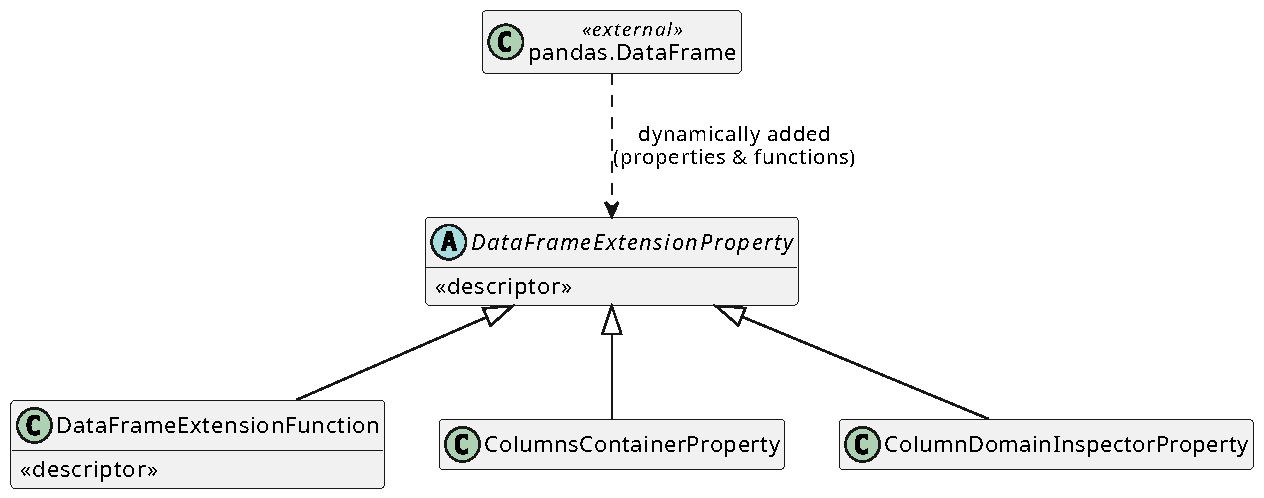
\includegraphics[width=\textwidth]{figures/uml/dataframe.pdf}
\caption{FairLib DataFrame Architecture}
\label{fig:df-uml}
\end{figure}

\section{Fairness Metrics}

The \textit{metrics} module embodies a rigorously structured architectural strategy aimed at reconciling computational performance with usability and extensibility. Central to its design is a clear separation of concerns that distinguishes the mathematical core of fairness metric computation from their operational integration within the overarching data analysis framework.

The adoption of a dual-layer architecture is motivated by the heterogeneity of the intended user base and use cases. On the one hand, data scientists require efficient and portable computational primitives that integrate seamlessly with \texttt{NumPy}-centric analytical workflows. On the other hand, end-users and applied practitioners benefit from higher-level abstractions that interface intuitively with custom data containers. To this end, core metric functions such as \texttt{disparate\_impact}, \texttt{statistical\_parity\_difference}, and \texttt{equality\_of\_opportunity} are implemented as independent, framework-agnostic operations over \texttt{NumPy} arrays. These low-level primitives are encapsulated within class-based wrappers (\texttt{DisparateImpact}, \texttt{StatisticalParityDifference}, etc.), which inherit from a common \texttt{Metric} base class, thereby enabling polymorphic usage and seamless integration with the DataFrame abstraction layer.

A particularly novel aspect of the design is the extension mechanism, which allows metric functionalities to be dynamically attached to \texttt{DataFrame} instances via a descriptor-based pattern, implemented through \texttt{DataFrameExtensionFunction}. In practice, this design allows users to invoke metrics via an object-oriented syntax (e.g., df.statistical\_parity\_difference()), which enhances discoverability and ease of use. This syntactic convenience significantly enhances the discoverability and accessibility of fairness evaluation tools, aligning with established paradigms in exploratory data analysis and interactive computing. A summary diagram can be read in Figure \ref{fig:metrics-uml}.

\begin{figure}
\centering
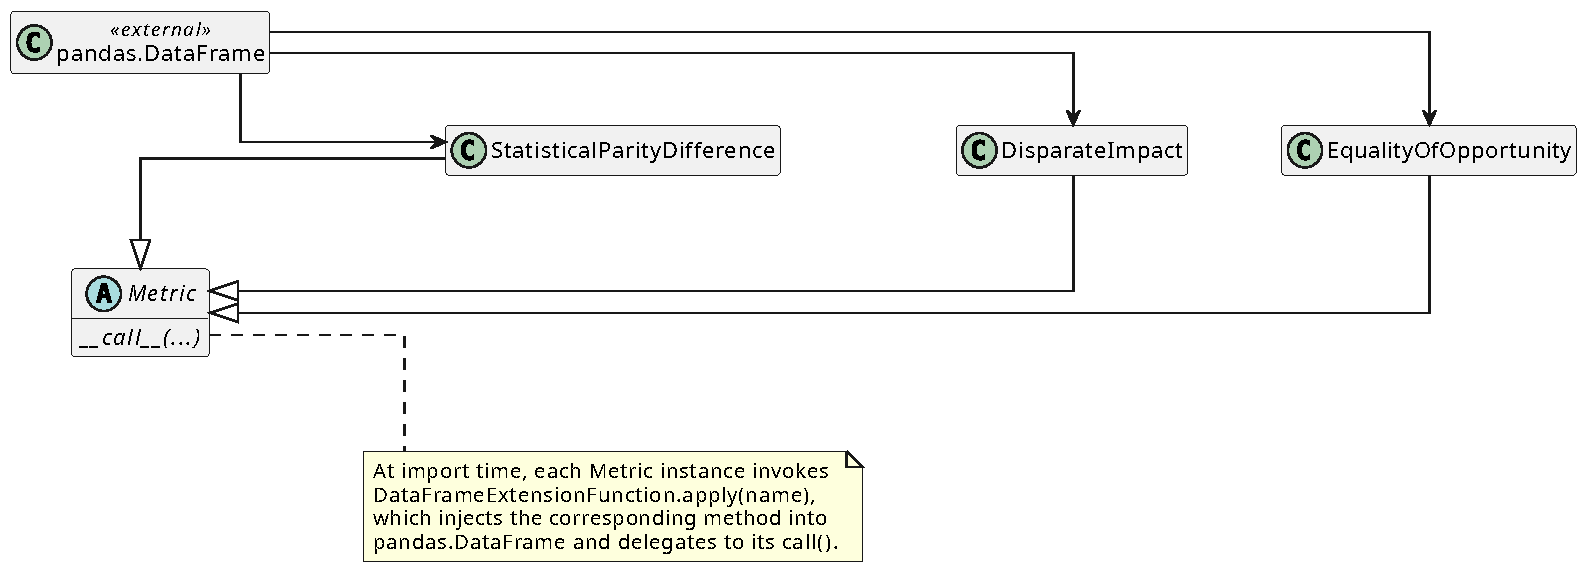
\includegraphics[width=\textwidth]{figures/uml/metrics.pdf}
\caption{FairLib Metrics Architecture}
\label{fig:metrics-uml}
\end{figure}

The inherent multidimensionality of fairness evaluation outcomes necessitated the introduction of dedicated data structures. In particular, the \texttt{DomainDict} class provides a semantically rich mapping layer that supports flexible querying across sensitive attributes, prediction targets, and their value combinations. This enables domain-aware operations such as selective retrieval by attribute names, partial assignments, or intersectional groupings, which are essential for nuanced fairness analyzes across diverse population strata.

Robust input validation and exception handling are implemented as first-class concerns within the library. The \texttt{check\_and\_setup} utility performs comprehensive precondition checks to ensure the dimensional alignment of sensitive attributes and outcome variables, issuing informative warnings in edge cases such as low group cardinality or missing categories. Furthermore, boundary conditions—such as metrics computed on empty demographic groups—are gracefully handled using \texttt{NaN} or infinite values, preserving the semantic consistency of results while avoiding runtime interruptions.

Finally, the metrics module supports multiple output modalities via the \texttt{as\_dict} parameter, which enables users to toggle between matrix-based representations optimized for numerical pipelines and dictionary-based formats that enhance readability and facilitate downstream processing (e.g., visualization or reporting). This dual-mode output capability reflects a deliberate design decision to serve both programmatic and interpretive aspects of fairness analysis within responsible machine learning workflows.


\subsection{Statistical Parity Difference}

Statistical Parity Difference represents a fundamental group fairness metric that quantifies the disparity in favorable outcome probabilities between privileged and unprivileged demographic groups. The theoretical foundation of this metric rests on the principle of demographic parity, which stipulates that a fair algorithmic system should produce equal acceptance rates across all protected groups, irrespective of the underlying ground truth distribution.

Mathematically, Statistical Parity Difference is formulated as:
\begin{equation}
\text{SPD} = P(\hat{Y}=1|S=\text{unprivileged}) - P(\hat{Y}=1|S=\text{privileged})
\end{equation}
where $\hat{Y}$ denotes the predicted outcome, $S$ represents the sensitive attribute, and the probabilities are computed over the respective demographic subgroups.

The implementation in FairLib follows a dual-layer architectural pattern, providing both a low-level functional interface and a high-level object-oriented wrapper. The core computational logic iterates through all unique combinations of target and sensitive attribute values, calculating group-specific acceptance rates through array masking operations. For each sensitive group $s$, the algorithm computes the privileged rate as $\frac{|{i: \hat{y}_i = t \land s_i = s}|}{|{i: s_i = s}|}$ and the unprivileged rate as $\frac{|{i: \hat{y}_i = t \land s_i \neq s}|}{|{i: s_i \neq s}|}$, where $t$ represents the target value. The implementation incorporates robust error handling for edge cases, including scenarios with empty subgroups, where infinite values are assigned to maintain mathematical consistency. The metric returns values in the range $[-1, 1]$, with zero indicating perfect fairness and values within $[-0.1, 0.1]$ generally considered acceptable in practical applications.

\subsection{Disparate Impact}

Disparate Impact constitutes a ratio-based fairness metric that emerged from legal frameworks, particularly the ``80\% rule" established in US anti-discrimination jurisprudence. This metric addresses the detection of indirect discrimination by measuring the relative likelihood of favorable outcomes between demographic groups, providing a multiplicative rather than additive perspective on fairness violations.

The mathematical formulation of Disparate Impact is expressed as:
\begin{equation}
\text{DI} = \frac{P(\hat{Y}=1|S=\text{unprivileged})}{P(\hat{Y}=1|S=\text{privileged})}
\end{equation}
This ratio-based approach offers intuitive interpretation: values below 1.0 indicate systematic disadvantage for the unprivileged group, while values above 1.0 suggest the opposite bias pattern.

The computational implementation mirrors the Statistical Parity Difference algorithm in its structural approach, utilizing the same group-wise probability estimation methodology. However, the critical distinction lies in the final aggregation step, where the unprivileged rate is divided by the privileged rate rather than subtracted. The implementation demonstrates careful attention to numerical stability, handling division-by-zero scenarios through appropriate infinite value assignments. The algorithm maintains consistency with legal standards by producing values in the range $[0, \infty)$, where perfect fairness corresponds to 1.0, and the legally acceptable threshold of 0.8 serves as a practical lower bound. Moreover, the FairLib implementation supports more complex scenarios, including multi-class targets and multiple sensitive attributes. It performs a comprehensive combinatorial evaluation across all target and attribute combinations, organizing the results in a structured DomainDict format. This design facilitates intersectional fairness analysis across diverse demographic categories.

\subsection{Equality of Opportunity}

Equality of Opportunity represents a more nuanced approach to algorithmic fairness that focuses specifically on ensuring equitable treatment among qualified individuals across demographic groups. This metric, grounded in the philosophical principle of meritocratic fairness, addresses scenarios where the primary concern is preventing discrimination against individuals who legitimately deserve favorable outcomes.

The theoretical framework centers on the concept of True Positive Rate (TPR) equalization, mathematically expressed as:
\begin{equation}
\text{EOO} = \text{TPR} {\text{privileged}} - \text{TPR} {\text{unprivileged}}
\end{equation}
where $\text{TPR}_{g} = P(\hat{Y}=1|Y=1, S=g)$ represents the true positive rate for demographic group $g$. This formulation ensures that qualified individuals (those with $Y=1$) have equal probabilities of receiving positive predictions regardless of their protected attribute status.

The implementation architecture in FairLib demonstrates sophisticated handling of the three-way relationship between true labels, predictions, and sensitive attributes. The algorithm employs boolean masking operations to identify qualified individuals within each demographic group, subsequently computing group-specific true positive rates through vectorized operations. The algorithm creates a boolean mask for the privileged group (e.g., $sensitive\_column == privileged\_value$) and its complement for the unprivileged group ($sensitive\_column != privileged\_value$). It then intersects these masks with the positive ground-truth mask ($target\_column == positive\_target$) to isolate qualified individuals in each group

The true positive rates are calculated as the ratio of correctly predicted positive cases to total positive cases within each group, with appropriate handling of empty sets through infinite value assignment. Unlike previous metrics, Equality of Opportunity requires an additional input—the ground truth labels (true outcomes)—making it suitable for post-hoc fairness evaluation after model training The metric produces values in the range $[-1, 1]$, where zero indicates perfect equality of opportunity, and the implementation supports flexible positive class specification through the positive\_target parameter, accommodating diverse labeling conventions across different application domains.

\section{Pre-Processing Algorithms}
The pre-processing module of FairLib implements a suite of algorithms designed to mitigate bias in datasets before model training. These algorithms transform the input data to reduce the influence of sensitive attributes, ensuring that subsequent learning processes are less affected by inherent biases.

The preprocessing module uses a consistent interface architecture (inspired by scikit-learn) designed specifically to work with FairLib’s enhanced DataFrame structure. The core interface consists of three primary methods: \texttt{fit()}, \texttt{transform()}, and \texttt{fit\_transform()}, see Figure \ref{fig:preprocessing-uml}. The \texttt{fit\_transform()} method serves as the primary interface that all preprocessing algorithms must implement, combining parameter learning and data transformation in a single operation. For algorithms requiring separate fitting and transformation phases, the \texttt{fit()} method learns parameters from the training data without modifying it, while \texttt{transform()} applies the learned transformation to new data. This separation enables efficient preprocessing of multiple datasets using the same learned parameters, which is particularly useful in train–test scenarios.

\begin{figure}
\centering
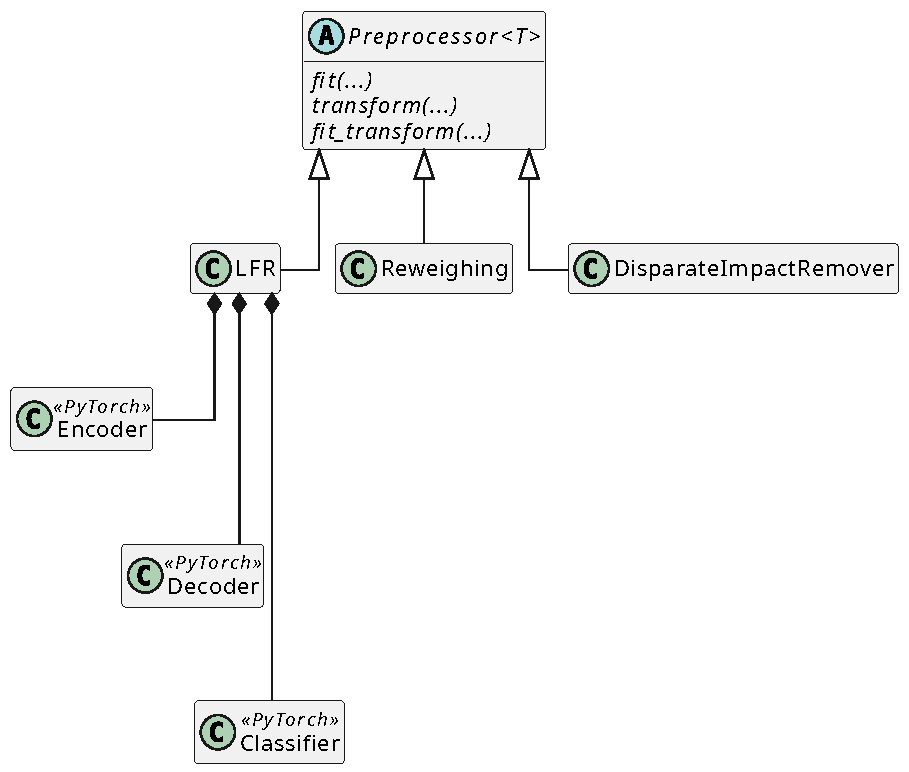
\includegraphics[width=\textwidth]{figures/uml/preprocessing.pdf}
\caption{FairLib Pre-processing Algorithms Architecture}
\label{fig:preprocessing-uml}
\end{figure}

All methods are designed to work exclusively with FairLib’s custom DataFrame, which extends the standard pandas DataFrame by preserving metadata for target and sensitive attributes. In particular, the DataFrame’s \texttt{unpack()} method automatically extracts the feature matrix, target labels, and sensitive attribute indices, while built-in validation ensures consistent data structure across algorithms.

\subsection{Reweighing}
The Reweighing algorithm implementation follows the statistical approach proposed by Kamiran and Calders \cite{kamiran2013quantifying}, where instance weights are computed to achieve statistical parity across different demographic groups. The core implementation centers around a static method \texttt{\_reweighing}, which calculates four distinct weight values corresponding to the combinations of privileged/unprivileged group status and favorable/unfavorable outcome.

The algorithm first validates the input DataFrame structure and identifies the target column. It then creates boolean masks for favorable and unfavorable outcomes using a private utility function \texttt{get\_favorable\_unfavorable\_masks}. For each combination of sensitive attribute value and target outcome, a weight is computed using the ratio formula 
\[ 
w \;=\; \frac{n_{\text{outcome}} \times n_{\text{group}}}{\,n_{\text{total}} \times n_{\text{joint}}\,}\,,
\] 
where $n_{\text{outcome}}$ is the total number of instances with the specified outcome (favorable or unfavorable) in the entire dataset, $n_{\text{group}}$ is the number of instances in the given demographic group (privileged or unprivileged), $n_{\text{total}}$ is the total number of instances in the dataset, and $n_{\text{joint}}$ is the number of instances that belong to both that group and that outcome category. The implementation also includes a specialized variant called \texttt{ReweighingWithMean}. This variant handles cases with multiple sensitive attributes by computing weights for each attribute independently and then averaging them, providing a more nuanced approach for intersectional fairness scenarios. The final transformed DataFrame includes a new \texttt{weights} column that can be directly used with scikit-learn classifiers via the \texttt{sample\_weight} parameter during training.

\subsection{Learning Fair Representations}
The Learning Fair Representations (LFR) algorithm is implemented as a deep neural network consisting of three interconnected components—an encoder, a decoder, and a classifier—constructed with PyTorch. The encoder network transforms the input features into a lower-dimensional “fair” representation, \textit{as illustrated in} Figure~\ref{fig:lfr_architecture}, using a three-layer fully connected architecture (input $\rightarrow$ 64 $\rightarrow$ 32 $\rightarrow$ latent\_dim) with ReLU activations; this 64–32 configuration is simply the library’s default and can be replaced by defining custom \texttt{Encoder}, \texttt{Decoder}, and \texttt{Classifier} modules that respect the required layer dimensions, making the entire LFR pipeline fully customizable. The decoder then attempts to reconstruct the original feature space from this representation using the symmetric architecture (latent\_dim $\rightarrow$ 32 $\rightarrow$ 64 $\rightarrow$ output\_dim), which can likewise be adapted to alternative depths or widths. 

\begin{figure}
\centering
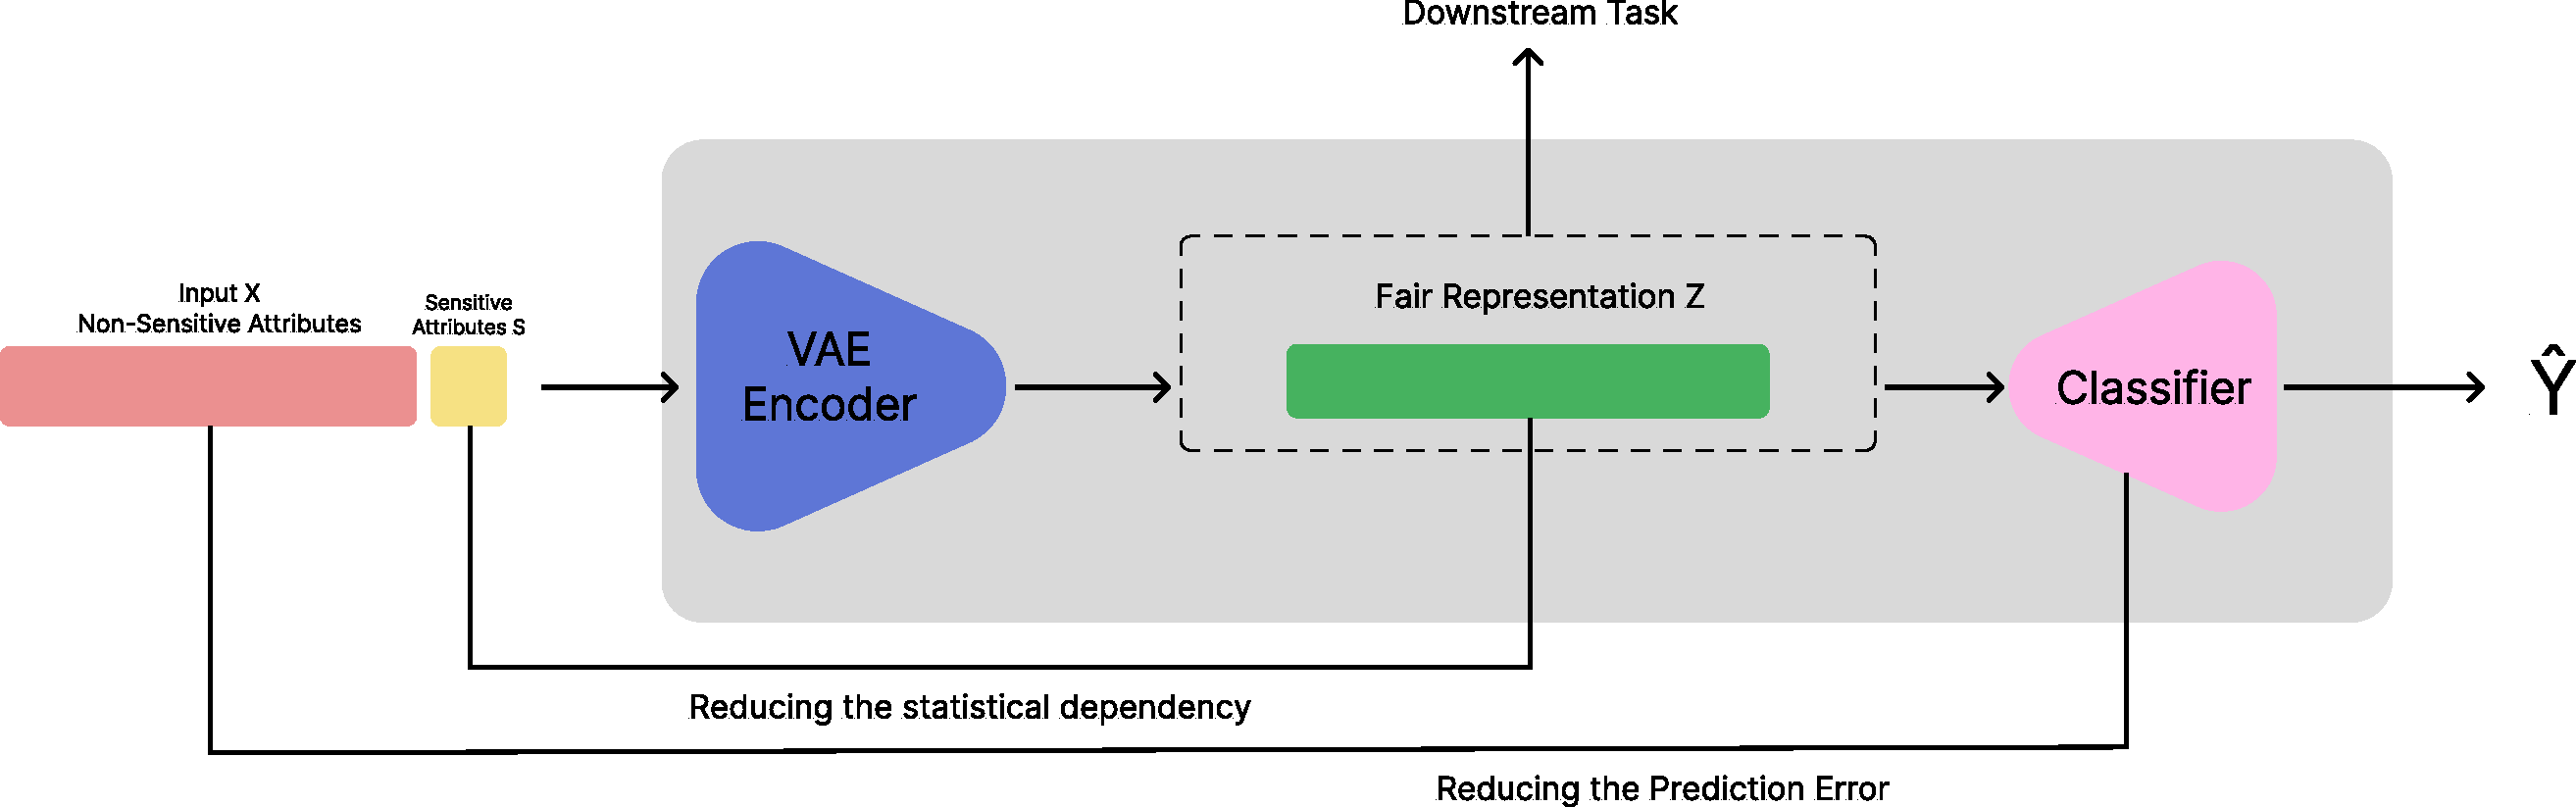
\includegraphics[width=\textwidth]{figures/lfr.pdf}
\caption{Architecture of the Learning Fair Representations (LFR) algorithm. The encoder compresses input features into a fair representation and the classifier predicts the target label from the fair representation \cite{TayebiAidaLfr}.}
\label{fig:lfr_architecture}
\end{figure}

Finally, a classifier component predicts the target label from the fair representation using a two-layer network that culminates in a sigmoid output unit for binary classification; like the encoder and decoder, this classifier can be freely re-implemented to suit specific tasks.

The training process optimizes a multi-objective loss function 
\[ 
L_{\text{total}} \;=\; \alpha_z\,L_z \;+\; \alpha_x\,L_x \;+\; \alpha_y\,L_y\,,
\] 
where $L_z$ is a fairness loss defined as the sum of squared differences between the mean representations of the protected and unprotected groups, $L_x$ is a reconstruction loss (measured as the mean squared error between the original features and their reconstructed counterparts), and $L_y$ is the binary cross-entropy loss for predicting the target. All three networks (encoder, decoder, and classifier) are trained jointly using the Adam optimizer, and input features are standardized via scikit-learn’s \texttt{StandardScaler} prior to training. During each forward pass, the encoder produces a fair representation, which the decoder uses to reconstruct the inputs and the classifier uses to predict the outcome. This joint training procedure ensures that the learned representations preserve predictive utility while minimizing sensitive attribute information. In particular, the fairness loss term $L_z$ serves as a statistical parity regularizer, encouraging the encoded representations to be independent of the sensitive attribute.

\subsection{Disparate Impact Remover}
The Disparate Impact Remover algorithm implements the fairness-aware “data repair” technique proposed by Feldman et al.~\cite{feldman2015certifyingremovingdisparateimpact}. This technique transforms feature distributions to achieve statistical parity across demographic groups through quantile-based distribution alignment.

In the implementation, the first step is to compute the empirical cumulative distribution function (CDF) for each feature within each sensitive attribute group. A helper function \texttt{\_make\_cdf} is used for this purpose; it returns a callable CDF for a given feature by sorting the feature values and enabling binary search lookup of quantile positions. During the fitting phase, the algorithm then constructs a quantile “map” for each feature as follows: it groups the data by sensitive attribute, establishes a common grid of quantile values (e.g., using \texttt{np.linspace} from 0 to 1), and computes the median feature value across all groups at each quantile level. These median values across quantiles form a reference distribution for the feature that represents a merged (fair) version of the original group-specific distributions.

In the transformation phase, each feature value $x$ is adjusted via this reference distribution. For a given data point, the algorithm first determines the quantile rank of $x$ within the CDF of its own sensitive group. It then uses linear interpolation (via \texttt{np.interp}) to map that quantile to the corresponding value in the reference (median) distribution. The resulting value $x_{\text{median}}$ is the fully “repaired” version of $x$ (i.e., the value $x$ would have in the median distribution). Finally, the algorithm computes the output as a weighted combination of the original and repaired values: 
\[ 
x_{\text{repaired}} \;=\; (1 - \lambda)\,x_{\text{original}} \;+\; \lambda\,x_{\text{median}}\,
\] 
Here $\lambda$ is the repair level parameter that controls the trade-off between fairness and data fidelity.

This approach makes the marginal distributions of each feature much more similar across different demographic groups, thereby reducing disparate impact, while still preserving some original data characteristics. The repair level $\lambda$ allows practitioners to balance between achieving complete distributional fairness ($\lambda = 1$, using only the median-aligned value) and preserving the original feature values ($\lambda = 0$, no adjustment). Additionally, the implementation preserves metadata consistency by keeping the same column names and retaining sensitive attribute information in the transformed DataFrame.

\section{In-Processing Algorithms}
The in-processing module of FairLib implements advanced fairness-aware machine learning algorithms by integrating fairness constraints directly into model training. This approach enables the simultaneous optimization of predictive accuracy and fairness objectives, allowing practitioners to achieve better trade-offs between these often competing goals. The implementation follows a modular design pattern, and all algorithms inherit from a common \texttt{Processor} base class that defines standard \texttt{fit()} and \texttt{predict()} methods. This abstraction ensures a consistent interface across different fairness algorithms and compatibility with FairLib’s DataFrame-based data handling system, making it easy to interchange in-processing mitigation methods within the library. A summary diagram can be read in Figure \ref{fig:inprocessing-uml}.

\begin{figure}
    \centering
    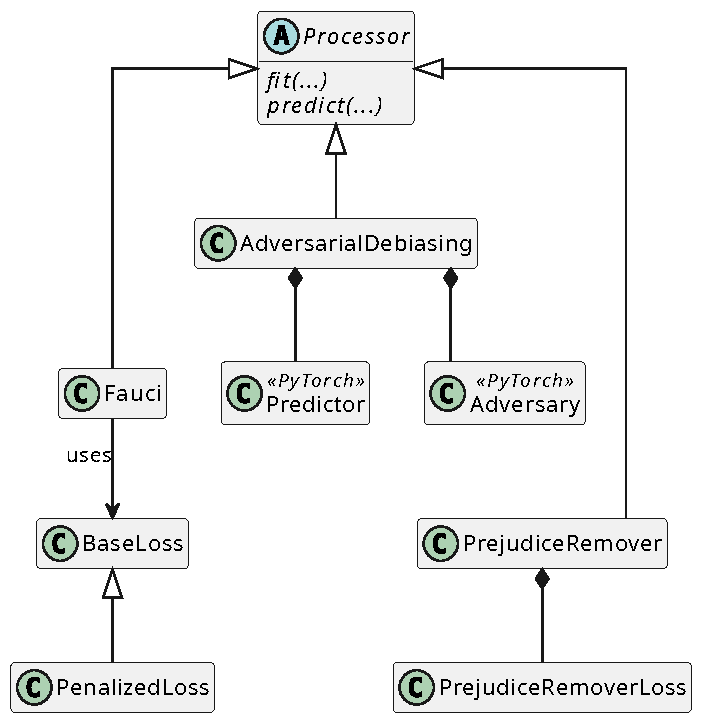
\includegraphics[width=\textwidth]{figures/uml/inprocessing.pdf}
    \caption{FairLib In-processing Algorithms Architecture}
    \label{fig:inprocessing-uml}
\end{figure}

\subsection{Adversarial Debiasing}
Building on the original Adversarial Debiasing framework of \cite{zhang2018mitigatingunwantedbiasesadversarial}, we adopt the architectural refinement proposed by \cite{beutel2017datadecisionstheoreticalimplications} in which the \emph{adversary consumes an intermediate hidden representation} rather than the predictor’s final logits.  This shift from an \textit{output-based} to a \textit{representation-based} adversarial signal encourages the predictor to remove sensitive information \emph{earlier} in the network and has been shown to yield stronger fairness guarantees while retaining predictive power.

The algorithm is implemented as a dual-network architecture in PyTorch, consisting of a predictor network and an adversarial network connected via a custom gradient-reversal layer.  At the heart of the implementation is the \texttt{GradientReversal} function, a custom autograd function that forwards inputs unchanged in the forward pass but in the backward pass multiplies the gradients by $-\lambda_{\text{adv}}$, thereby reversing and scaling them by the factor $\lambda_{\text{adv}}$.  

The predictor network is a three-layer feed-forward model: each hidden layer applies batch normalization (\texttt{BatchNorm1d}) before a linear transformation, followed by a ReLU activation and dropout (default drop rate $0.3$) for regularization.  Crucially, it returns both the task logits and the hidden representation $\mathbf{h}$ that serves as input to the adversary.  Both the predictor and the adversary can be replaced with custom \texttt{nn.Module}s, provided they share a compatible interface: (i) the predictor must expose a representation whose dimensionality matches the adversary’s input size, and (ii) both modules must return logits suitable for their respective loss functions.

An example of this architecture is shown in Figure~\ref{fig:adversarial_debiasing}.
\begin{figure}
  \centering
  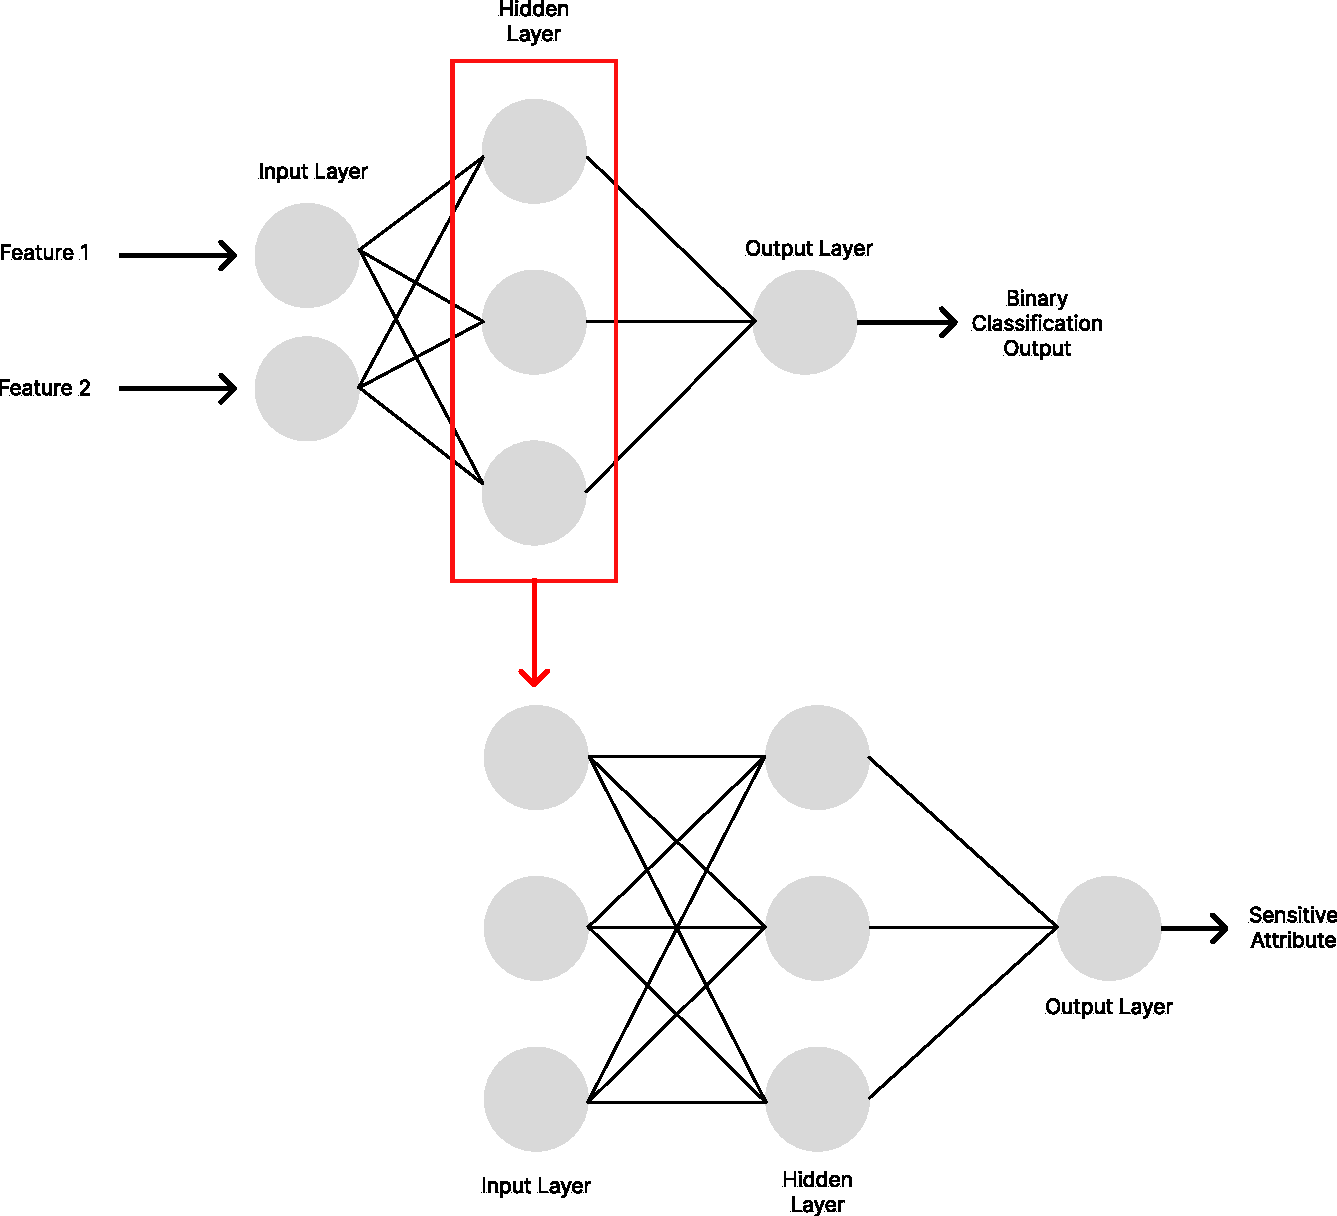
\includegraphics[width=0.9\textwidth]{figures/adversarial_debiasing.pdf}
  \caption{Adversarial Debiasing architecture: a predictor network learns to make predictions while an adversarial network attempts to predict the sensitive attribute from the predictor's \emph{internal} representation, following the hidden-layer strategy.}
  \label{fig:adversarial_debiasing}
\end{figure}

This flexibility allows practitioners to experiment with deeper, convolutional, or transformer-based architectures without changing the training loop.  The adversarial network mirrors the predictor's architecture (including batch normalization and dropout) but employs LeakyReLU activations in its hidden layers.  During training, an alternating optimization strategy is employed: in each iteration, the adversary is first updated for a fixed number of steps (\texttt{adv\_steps}) to better predict the sensitive attribute from $\mathbf{h}$ (with predictor parameters frozen), and then the predictor is updated (via the gradient-reversal mechanism) to minimize its primary prediction loss while \emph{maximizing} the adversary’s loss.  This effectively forces the predictor to learn representations that confound the adversary, thereby promoting fairness at the representation level.  To stabilize training, gradient clipping (max-norm $1.0$) is applied to both networks, and optimization is performed with AdamW (including weight decay).  Hyperparameters such as learning rates, batch size, the number of adversary steps, and the critical $\lambda_{\text{adv}}$ parameter controlling the fairness–accuracy trade-off remain fully configurable.

\subsection{FaUCI: Fairness Under Constrained Injection}
The \textbf{FaUCI} (Fairness Under Constrained Injection) algorithm incorporates fairness metrics directly into the loss function as regularization terms. It is implemented through a modular loss architecture that seamlessly integrates with standard PyTorch training workflows. In particular, a hierarchical loss design is used: a base loss (e.g. cross-entropy for classification) is encapsulated by a \texttt{BaseLoss} class, and a \texttt{PenalizedLoss} subclass extends this by adding a fairness regularization term. The total loss at each training step is computed as a weighted sum of the base loss and the fairness penalty:

\begin{equation}
    L_{\text{total}} \;=\; (1 - w)\,L_{\text{base}} \;+\; w\,L_{\text{fairness}},
\end{equation}

where $w$ is the regularization weight that controls the trade-off between accuracy and fairness. The fairness penalty leverages a pluggable metric system (implemented in \texttt{\_torch\_metrics.py}) supporting metrics such as Statistical Parity Difference (SPD) and Disparate Impact (DI). These metrics are computed on each mini-batch during training to provide an on-the-fly estimate of unfairness. For example, the SPD metric is calculated as the absolute difference in positive outcome probability between the protected and unprotected groups, while the DI metric is the ratio of these probabilities. Both metrics are efficiently computed using the model’s predictions for the current mini-batch, with a small epsilon (e.g. $10^{-7}$) added to probability estimates to ensure numerical stability (avoiding division by zero or undefined log values). The \texttt{FaUCI} class serves as the main processor for this algorithm, wrapping an arbitrary PyTorch model and managing the training loop via a flexible interface. It allows users to specify custom optimizers, base loss functions, and fairness metrics (along with the regularization weight $w$). During training, the sensitive attribute values for each batch are passed into the loss computation (via a property injection mechanism) so that the fairness metric can be evaluated for that batch’s predictions. The implementation supports a range of hyperparameters including the number of epochs, batch size, and the regularization weight $w$, making FaUCI a versatile framework for exploring different fairness–accuracy trade-offs.

\subsection{Prejudice Remover}
The Prejudice Remover algorithm is implemented via a mutual-information-based regularization framework, which explicitly penalizes the model for encoding statistical dependence between its predictions and the sensitive attribute. The core of this approach is a \texttt{PrejudiceRemoverLoss} that augments the standard prediction loss with a mutual information ($MI$) penalty term:
\begin{equation}
    L_{\text{total}} = L_{\text{base}} \;+\; \eta \cdot MI(\hat{Y}, S)\,
\end{equation}
where $\eta$ is a hyperparameter controlling the strength of the fairness regularization. Here $MI(\hat{Y}, S)$ measures the mutual information between the model’s output $\hat{Y}$ and the sensitive attribute $S$, which is zero if the predictions are independent of $S$. In practice, this mutual information is estimated on each mini-batch by computing the joint distribution $P(\hat{Y}, S)$ and the marginal distributions $P(\hat{Y})$ and $P(S)$ from the batch’s predictions and labels. The implementation calculates group-conditional probabilities (such as $P(\hat{Y}=1 \mid S=0)$ and $P(\hat{Y}=1 \mid S=1)$) by averaging the model’s predicted probabilities for the positive class within each sensitive group in the batch. Using these, it obtains estimates of $P(\hat{Y}=1, S=0)$, $P(\hat{Y}=1, S=1)$, etc., for all four combinations of binary outcome and sensitive value. To prevent numerical issues (e.g. $\log(0)$), a small epsilon ($10^{-8}$) is added to each probability estimate. The mutual information penalty is then computed as the \textbf{Kullback–Leibler} divergence between the joint and product-of-marginals distributions:
\begin{equation}
    MI(\hat{Y}, S) \;\approx\; \sum_{y\in\{0,1\}} \sum_{s\in\{0,1\}} P(\hat{Y}=y,\;S=s)\; \log \frac{P(\hat{Y}=y,\;S=s)}{\,P(\hat{Y}=y)\,P(S=s)\,}\,
\end{equation}
which corresponds to summing over the four possible $(y, s)$ combinations in the binary case. The \texttt{PrejudiceRemover} class integrates this loss into a PyTorch training pipeline, allowing flexible model architectures via dependency injection and automatically converting FairLib’s DataFrame inputs into tensors for training. The training routine ensures proper gradient flow through the mutual information term (so that the model’s predictions are influenced by the penalty), and it supports both binary cross-entropy and mean squared error as the base loss (depending on the prediction task). To help practitioners monitor progress, the implementation includes extensive logging of metrics, tracking the model’s predictive performance as well as fairness indicators (such as the estimated $MI$ or group outcome differences) at each epoch. This mutual-information regularization approach (originally proposed by Kamishima et al. \cite{kamishima2012prejudiceremoverregularizer}) encourages the model to produce fairer predictions by explicitly discouraging any measurable dependency between $\hat{Y}$ and $S$.

\chapter{Evaluation and Results}


This chapter presents an empirical evaluation of the proposed Python library for algorithmic fairness. We analyze its behavior along four complementary axes: \emph{verbosity of the API}, \emph{ease of use}, \emph{seamless integration within existing machine--learning pipelines}, and \emph{quantitative impact on fairness metrics}. The goal is to provide a comprehensive view of the trade--offs introduced by the library and to validate its practical utility.


\section{Verbosity Analysis}
In this section we quantify the amount of code required to express common fairness workflows using the library such as computing fairness metrics, applying pre-processing algorithms, and integrating in-processing techniques. 


\subsection{Metrics}
The \texttt{FairLib} library provides a streamlined interface for computing a wide variety of fairness metrics, allowing for efficient integration into experimental workflows. In particular, it supports the evaluation of group fairness criteria with minimal coding effort. The code snippet \ref{lst:metrics_example} illustrates how to compute key metrics such as Statistical Parity Difference, Disparate Impact, and Equality of Opportunity, which are commonly used to assess the presence of bias in classification models.

\lstinputlisting[caption={Example Python script for computing fairness metrics}, label={lst:metrics_example}]{listings/results/metrics.py}

Only twelve lines-eight if we omit comments-are needed to progress from raw tabular data to a structured fairness report. Each metric call returns a dictionary. The library automatically infers the target and sensitive attributes from the DataFrame metadata, eliminating the need for explicit parameter passing. This significantly reduces cognitive load and potential errors in specifying these identifiers.

\subsection{Pre-processing Algorithms}
The library's pre-processing algorithms are designed to be easily applied to datasets with minimal boilerplate code. The code snippet \ref{lst:preprocessing_example} demonstrates how to apply the Reweighing algorithm, which adjusts instance weights to mitigate bias in classification tasks. The example shows how to instantiate the algorithm, fit it to the data, and transform the dataset in just a few lines of code.

\lstinputlisting[caption={Example Python script for applying the Reweighing pre-processing algorithm}, label={lst:preprocessing_example}]{listings/results/preprocessing.py}

Support for \textbf{multiple sensitive attributes} enables intersectional fairness analysis within the library’s framework. Instance weights are automatically computed and appended to the dataset, allowing for seamless integration with scikit-learn classifiers via the \texttt{sample\_weight} parameter.

The Reweighing algorithm is particularly useful for addressing disparities in classification outcomes by adjusting the weights of instances based on their sensitive attributes. The library's design allows users to easily switch between different pre-processing techniques, such as Learning Fair Representations or Disparate Impact Remover, with minimal code changes.

\subsection{In-processing Algorithms}
The in-processing algorithms in FairLib are designed to be easily integrated into existing machine learning workflows. The code snippet \ref{lst:inprocessing_example} illustrates how to apply the Adversarial Debiasing algorithm, which trains a model to make predictions while simultaneously minimizing bias with respect to sensitive attributes.

\lstinputlisting[caption={Example Python script for applying the Adversarial Debiasing in-processing algorithm}, label={lst:inprocessing_example}]{listings/results/inprocessing.py}

The example shows how to instantiate the Adversarial Debiasing processor, fit it to the training data, and make predictions with just a few lines of code. The library's design allows users to easily switch between different in-processing techniques, such as FaUCI or Prejudice Remover, with minimal code changes.


\section{Integration into Existing Pipelines}
This section explores how the library can be embedded into pre--existing scikit--learn\,/\,PyTorch pipelines with minimal refactoring. We discuss interoperability with data preprocessing stages, hyperparameter optimization loops, and model persistence mechanisms.

\subsection{Preprocessing Integration}
The library's preprocessing algorithms can be seamlessly integrated into existing data pipelines. The code snippet \ref{lst:unfair_preprocessing} shows a basic example of binary classification, without the application of any fairness algorithms.

\lstinputlisting[caption={Example Python script of a classification process without application of fairness}, label={lst:unfair_preprocessing}]{listings/integrations/preprocessing.py}

In contrast, the code snippet \ref{lst:fair_preprocessing} demonstrates how to apply the LFR pre-processing algorithm to the same dataset, adjusting instance weights based on sensitive attributes.

\lstinputlisting[caption={Example Python script of a classification process with application of fairness}, label={lst:fair_preprocessing}]{listings/integrations/fair_preprocessing.py}

This example illustrates how the library's preprocessing algorithms can be easily integrated into existing data pipelines, allowing users to apply fairness techniques without significant changes to their codebase. The preprocessing step is performed before model training, ensuring that the model learns from a fair representation of the data.

\subsection{In-processing Integration}

The library's in-processing algorithms can be integrated into existing model training workflows with minimal code changes. The code snippet \ref{lst:unfair_inprocessing} shows a basic example of training a PyTorch model without applying any fairness techniques.

\lstinputlisting[caption={Example Python script of a PyTorch model training process without application of fairness}, label={lst:unfair_inprocessing}]{listings/integrations/inprocessing.py}

In contrast, the code snippet \ref{lst:fair_inprocessing} demonstrates how to apply FaUCI in-processing algorithm during model training.

\lstinputlisting[caption={Example Python script of a PyTorch model training process with application of fairness}, label={lst:fair_inprocessing}]{listings/integrations/fair_inprocessing.py}

This example illustrates how the library's in-processing algorithms can be easily integrated into existing model training workflows, allowing users to apply fairness techniques without significant changes to their codebase. The in-processing step is performed during model training, ensuring that the model learns to make fair predictions while optimizing for accuracy.

\section{Effect of Mitigation on Fairness}
\subsection{Experimental Setup}
We describe the datasets, target variables, protected attributes, and evaluation protocol employed to measure fairness both prior to and after applying the library's pre--processing and in--processing algorithms. For this evaluation, we use the Adult Income dataset \cite{adultDataset}, which contains demographic information about individuals and whether they earn more than \$50,000 per year. The sensitive attribute is \texttt{sex}, and the target variable is \texttt{income} (binary classification: income $\leq$ \$50,000 vs. income $>$ \$50,000). The dataset is split into training and test sets, with the training set used for model fitting and the test set for evaluation.

The evaluation protocol, for \textbf{pre-processing algorithms}, consists of the following steps:
\begin{enumerate}
    \item Compute fairness metrics (Statistical Parity Difference, Disparate Impact) on the original dataset.
    \item Apply pre-processing algorithms (Reweighing, Learning Fair Representations, Disparate Impact Remover) to the training set.
    \item Train a classifier (logistic regression) on the transformed training set.
    \item Compute fairness metrics on the test set after applying the pre-processing algorithms.
\end{enumerate}

For \textbf{in-processing algorithms}, the evaluation protocol consists of:
\begin{enumerate}
    \item Compute fairness metrics (Statistical Parity Difference, Disparate Impact) on the original dataset.
    \item Train a classifier (Neural Network) with in-processing algorithms (Adversarial Debiasing, FaUCI, Prejudice Remover) integrated into the training loop.
    \item Compute fairness metrics on the test set after training with in-processing algorithms.
\end{enumerate}

\subsection{Results Summary}
A concise presentation of key numerical results, focusing on disparity measures (e.g., Statistical Parity Difference, Disparate Impact) and accuracy.
\subsubsection{Pre-processing Algorithms Results}
The results of applying pre-processing algorithms to the Adult Income dataset are summarized in 3 figures. Figure \ref{fig:baseline_results} shows the accuracy of the baseline model and the models trained after applying pre-processing algorithms. The accuracy is computed on the test set of the Adult Income dataset.
Figure \ref{fig:preprocessing_results} shows the Statistical Parity Difference (SPD) for the baseline model and the models trained after applying pre-processing algorithms. The SPD is computed on the test set of the Adult Income dataset. Figure \ref{fig:preprocessing_results_di} shows the Disparate Impact (DI) for the baseline model and the models trained after applying pre-processing algorithms. The DI is computed on the test set of the Adult Income dataset.

\begin{figure}
    \centering
    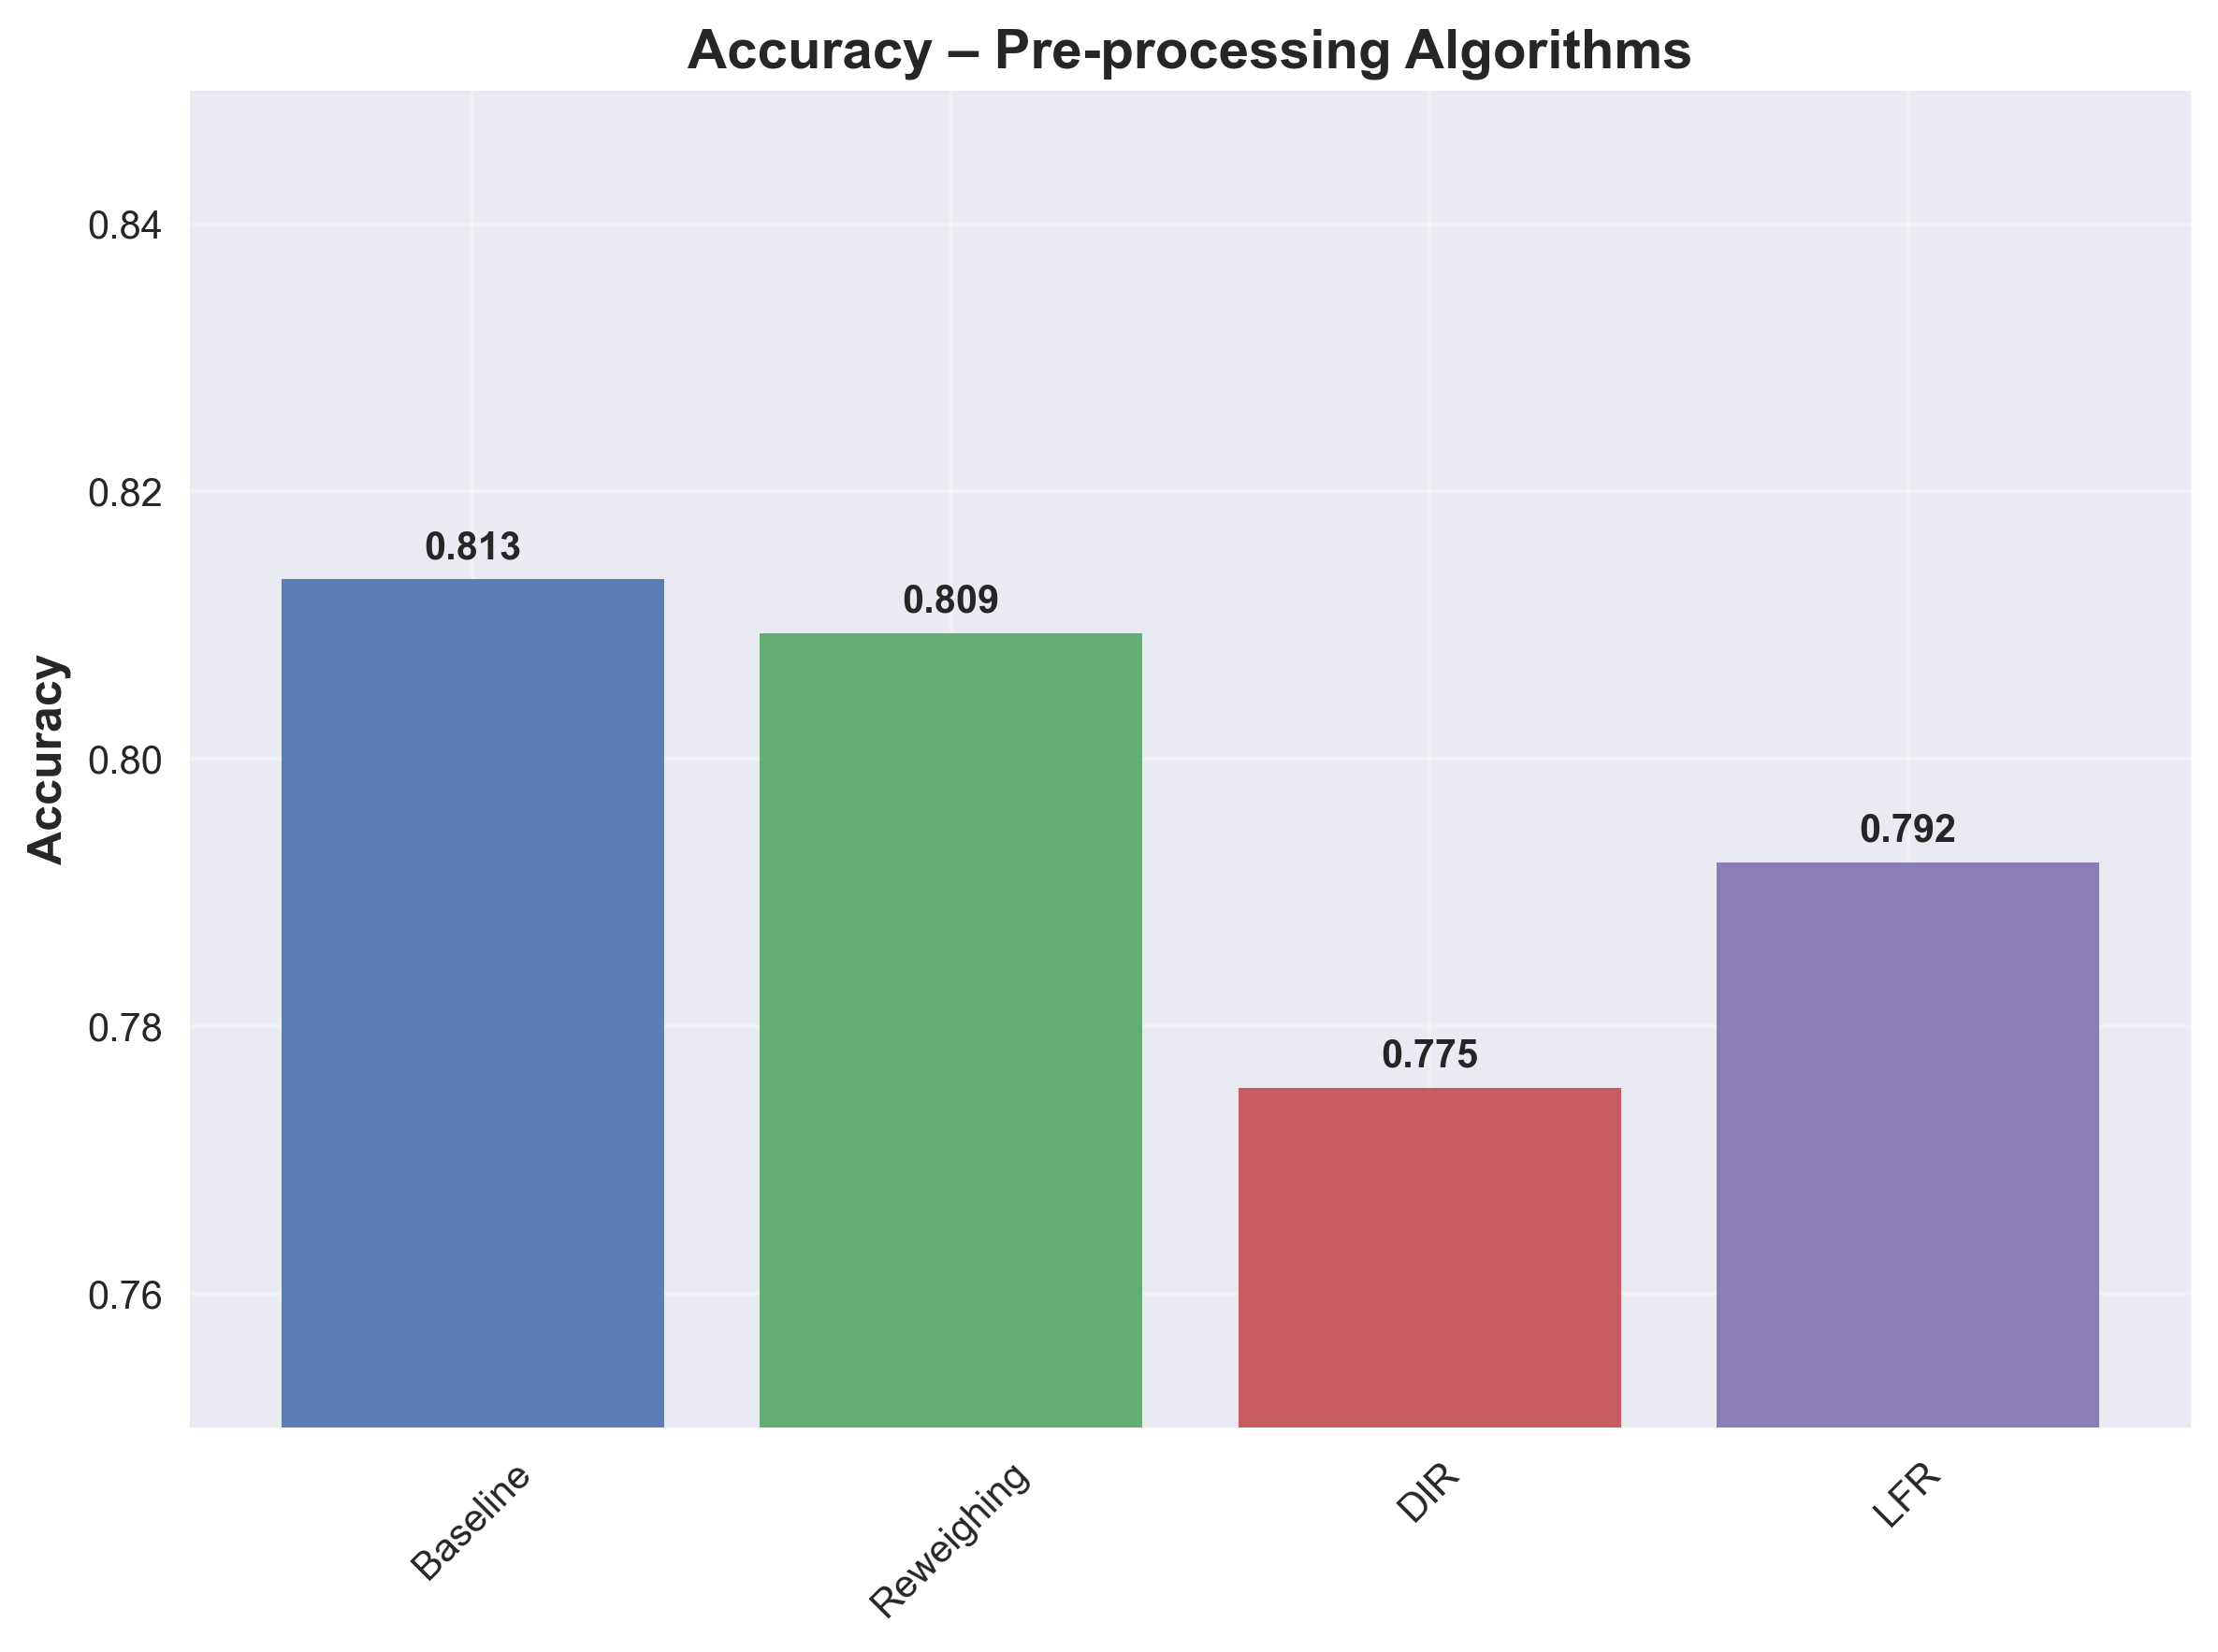
\includegraphics[width=\textwidth]{figures/preprocessing_results/preprocessing_accuracy_comparison.png}
    \caption{Accuracy score for the baseline model and the models trained after applying pre-processing algorithms. The accuracy is computed on the test set of the Adult Income dataset.}
    \label{fig:baseline_results}
\end{figure}

\begin{figure}
    \centering
    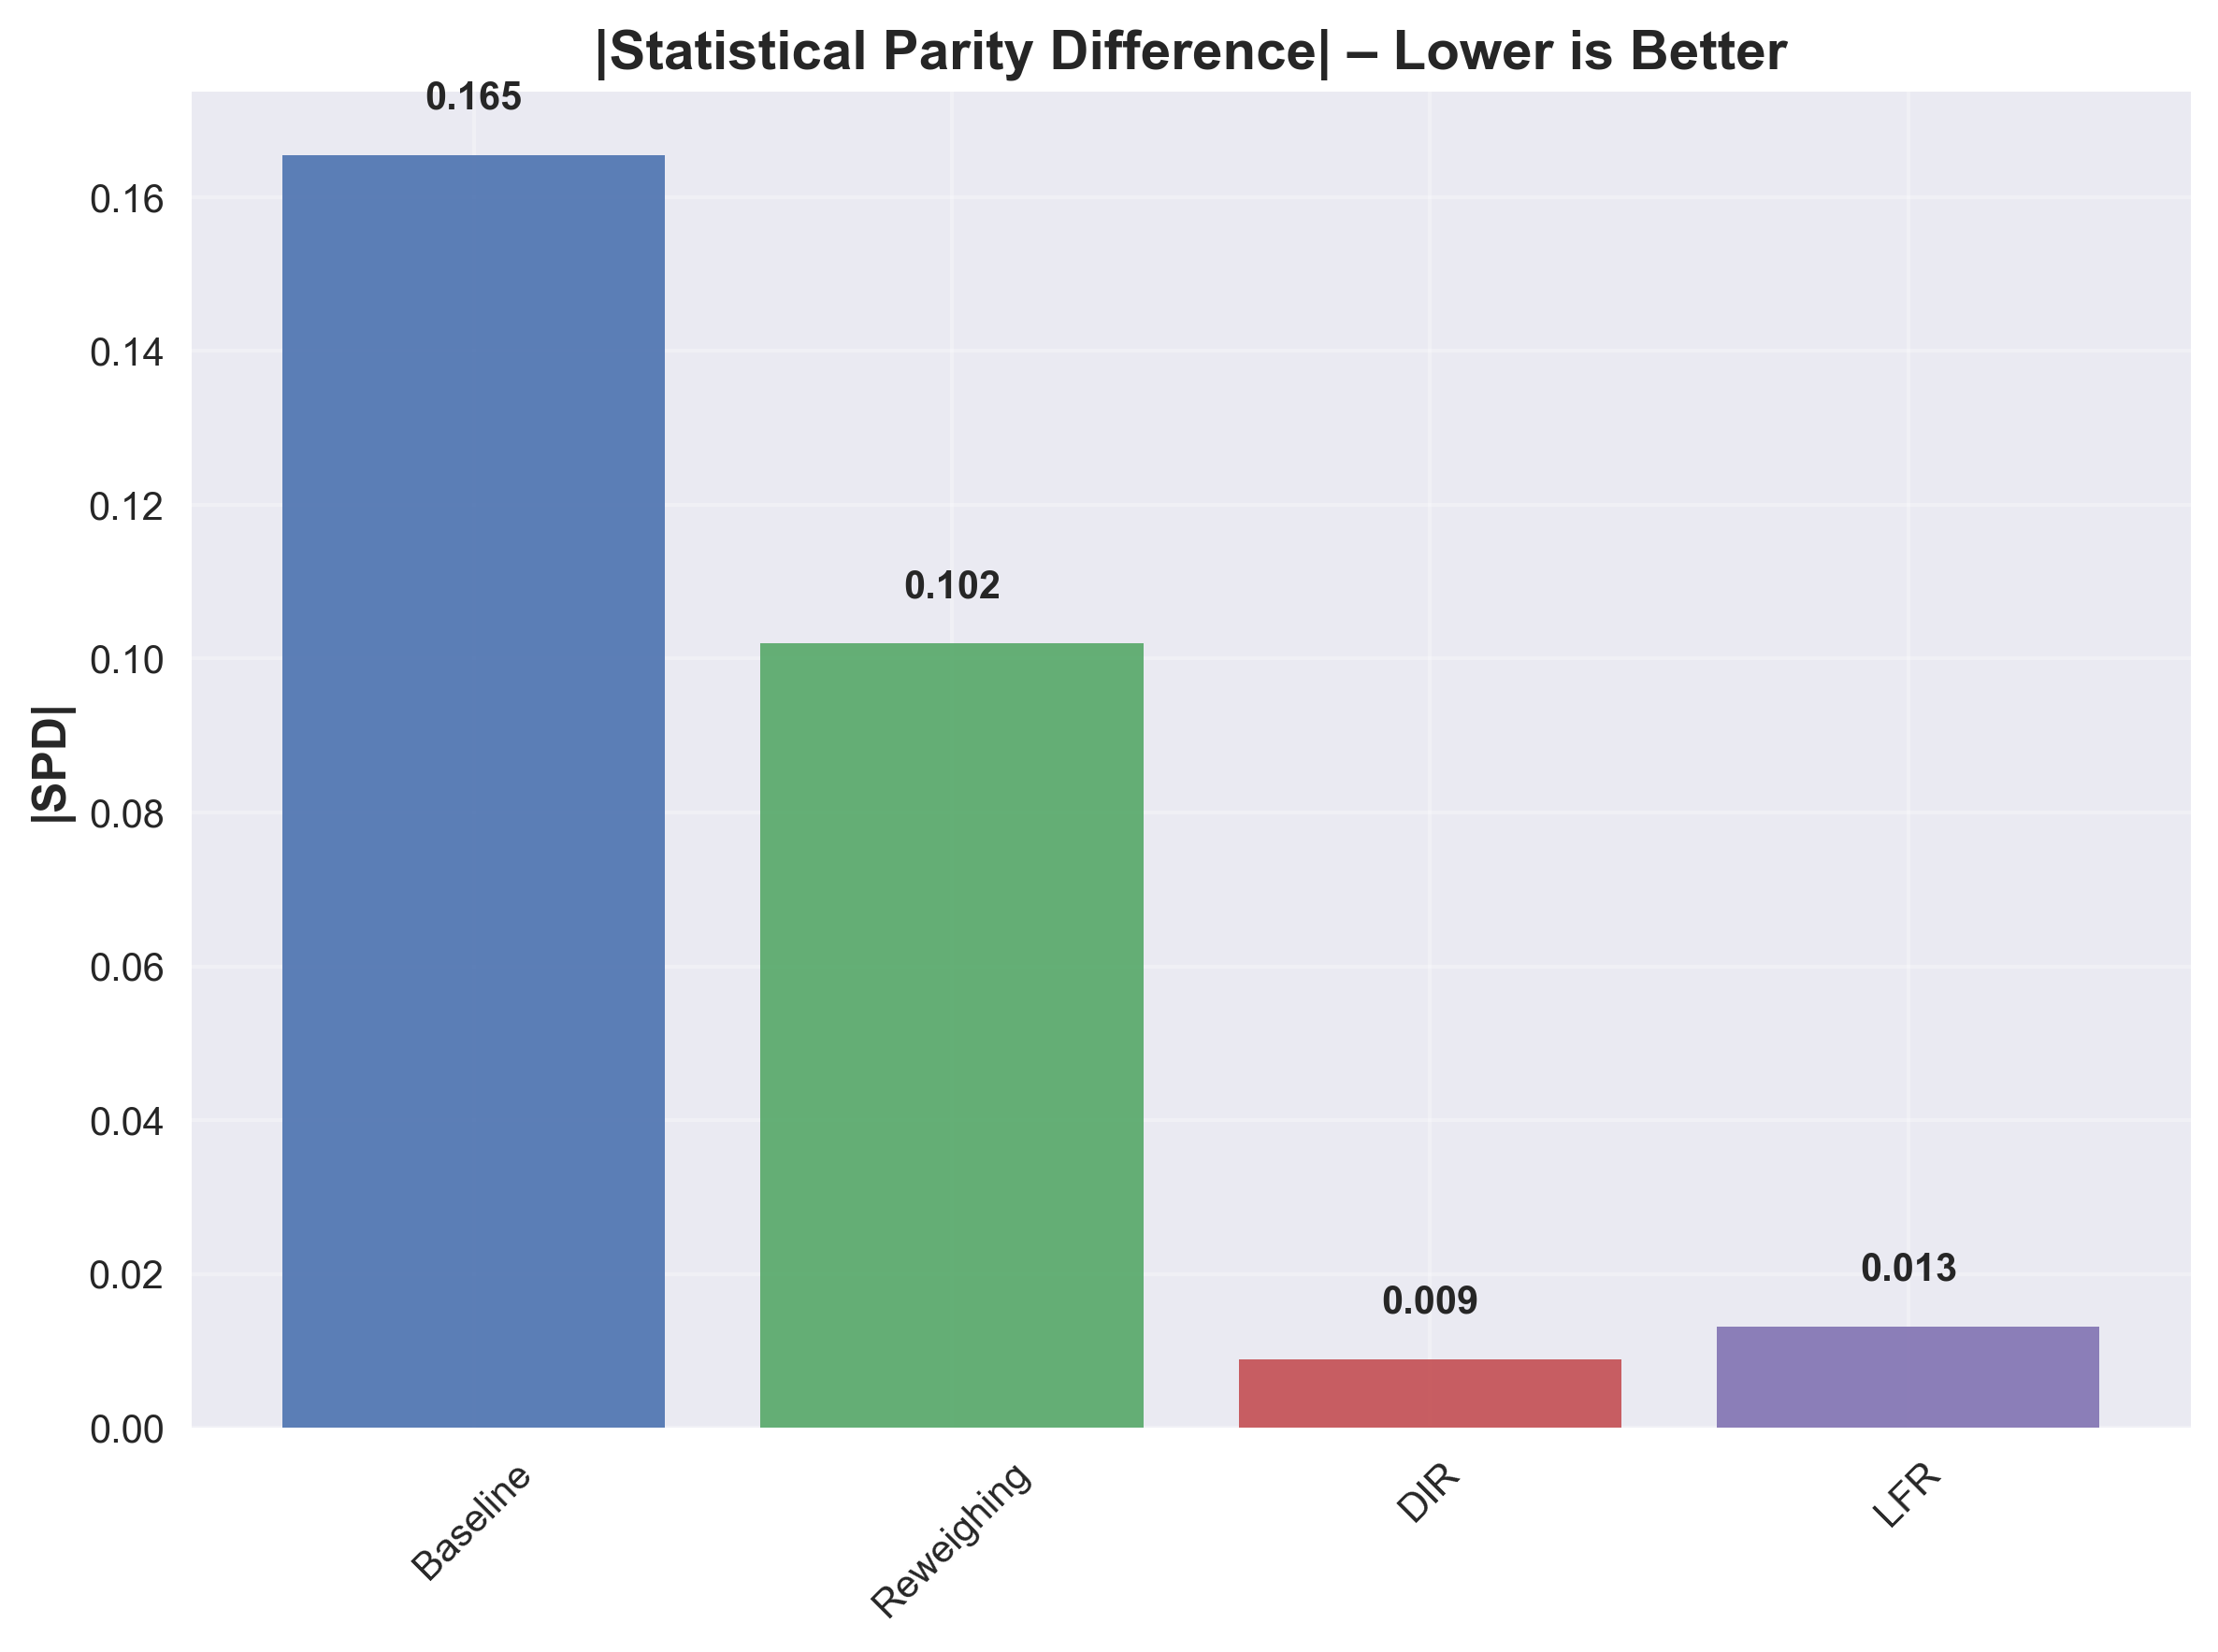
\includegraphics[width=\textwidth]{figures/preprocessing_results/preprocessing_spd_comparison.png}
    \caption{Statistical Parity Difference (SPD) for the baseline model and the models trained after applying pre-processing algorithms. The SPD is computed on the test set of the Adult Income dataset.}
    \label{fig:preprocessing_results}
\end{figure}

\begin{figure}
    \centering
    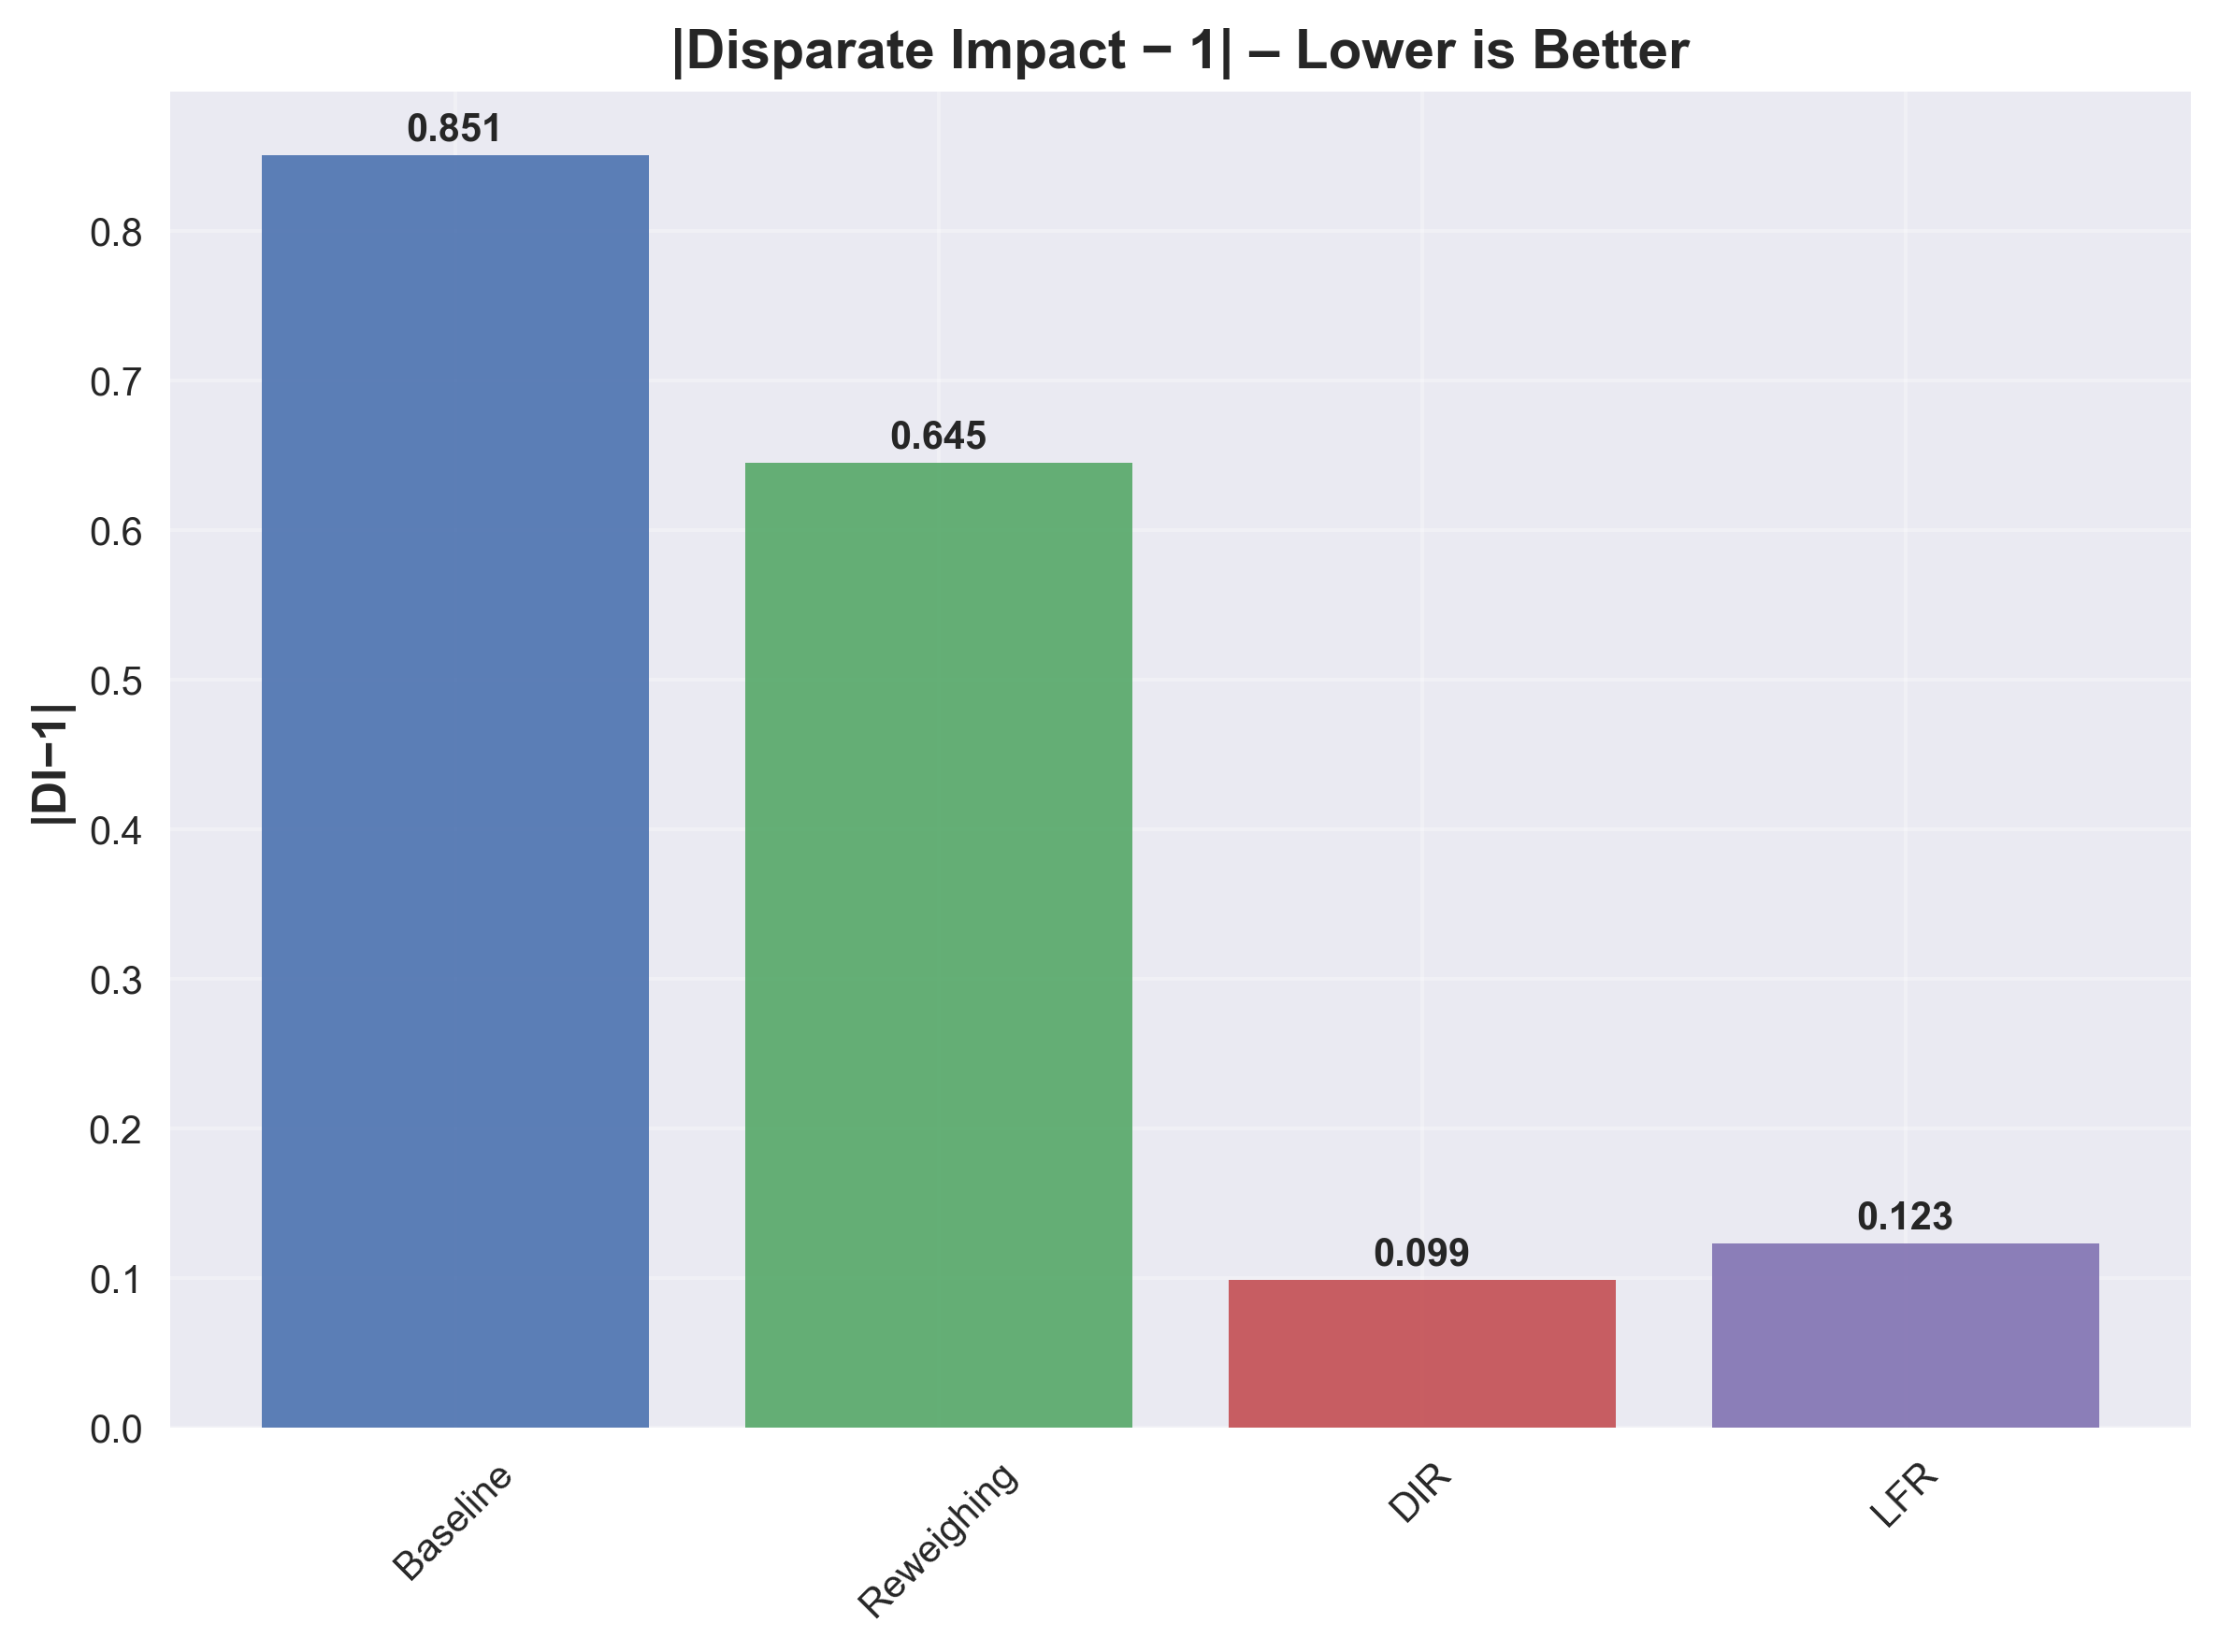
\includegraphics[width=\textwidth]{figures/preprocessing_results/preprocessing_di_comparison.png}
    \caption{Disparate Impact (DI) for the baseline model and the models trained after applying pre-processing algorithms. The DI is computed on the test set of the Adult Income dataset.}
    \label{fig:preprocessing_results_di}
\end{figure}

From the results obtained by applying the algorithms in the pre-processing module, we observe that all algorithms successfully reduce the Statistical Parity Difference (SPD) and Disparate Impact (DI) metrics compared to the baseline model.

\subsubsection{In-processing Algorithms Results}

The results of applying in-processing algorithms to the Adult Income dataset are summarized in 3 figures. Figure \ref{fig:baseline_results_inprocessing} shows the accuracy of the baseline model and the models trained after applying in-processing algorithms. The accuracy is computed on the test set of the Adult Income dataset.
Figure \ref{fig:inprocessing_results} shows the Statistical Parity Difference (SPD) for the baseline model and the models trained after applying in-processing algorithms. The SPD is computed on the test set of the Adult Income dataset. Figure \ref{fig:inprocessing_results_di} shows the Disparate Impact (DI) for the baseline model and the models trained after applying in-processing algorithms. The DI is computed on the test set of the Adult Income dataset.

\begin{figure}
    \centering
    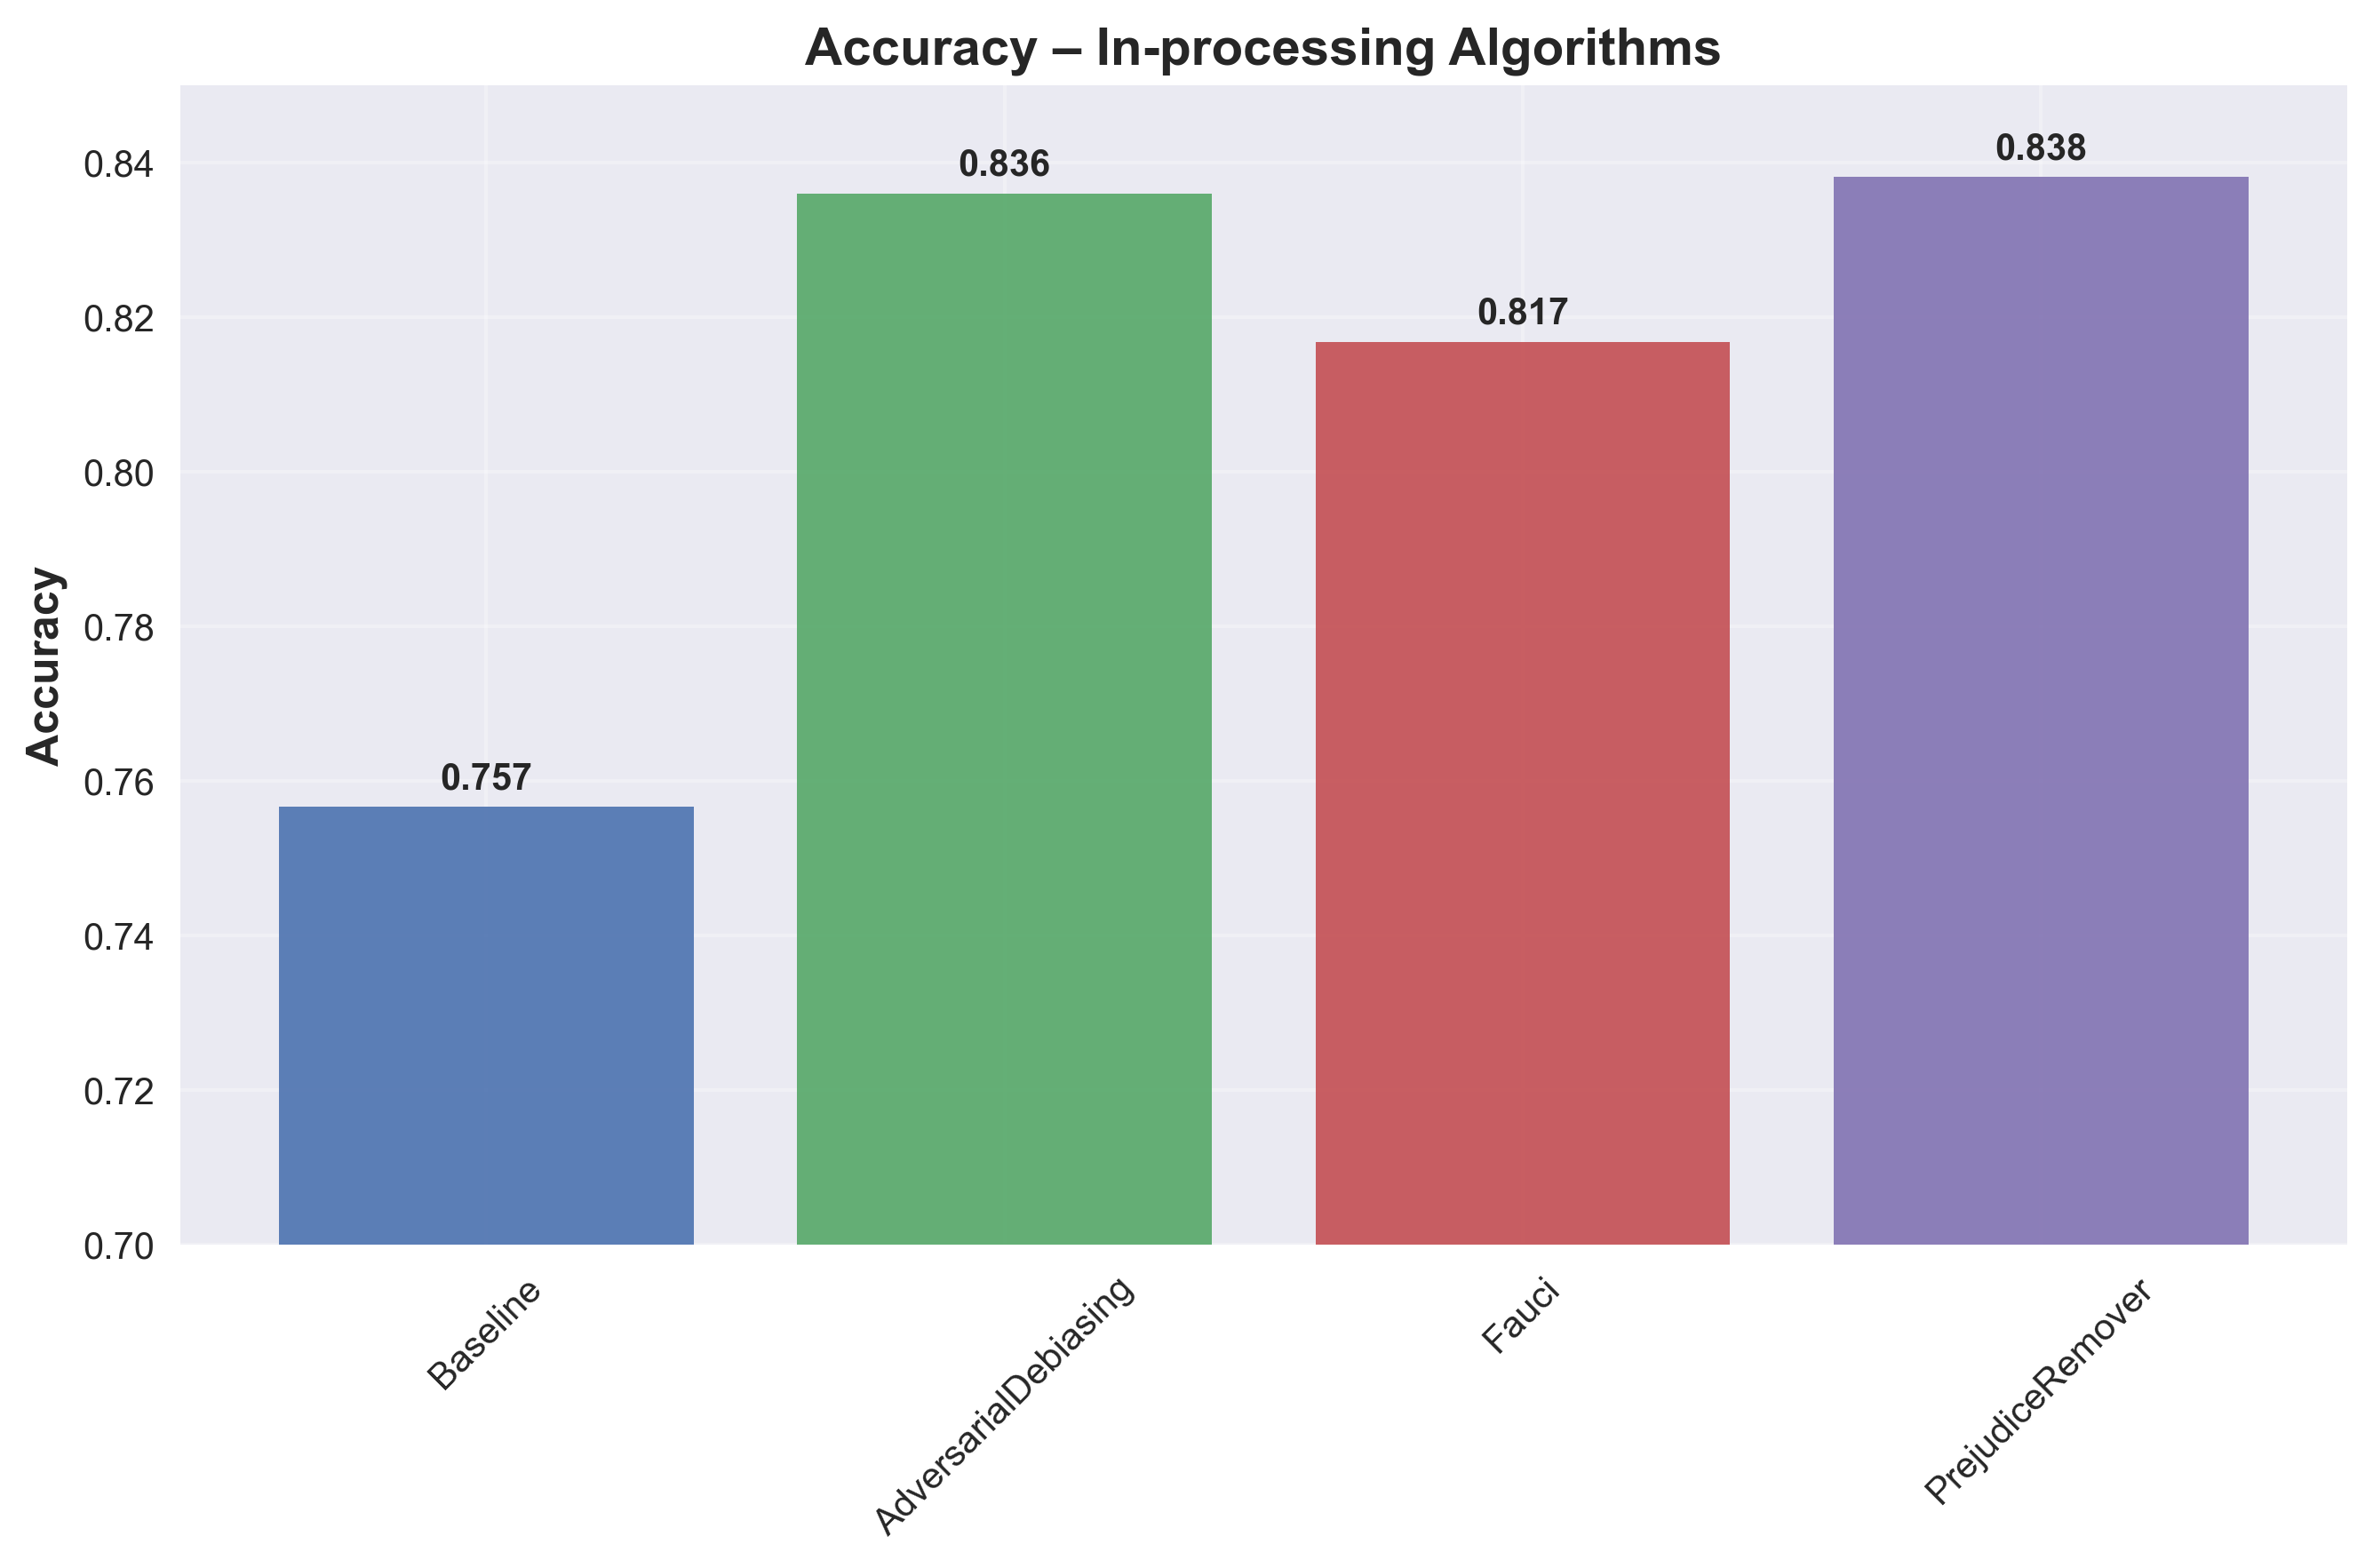
\includegraphics[width=\textwidth]{figures/inprocessing_results/inprocessing_accuracy_comparison.png}
    \caption{Accuracy score for the baseline model and the models trained after applying in-processing algorithms. The accuracy is computed on the test set of the Adult Income dataset.}
    \label{fig:baseline_results_inprocessing}
\end{figure}

\begin{figure}
    \centering
    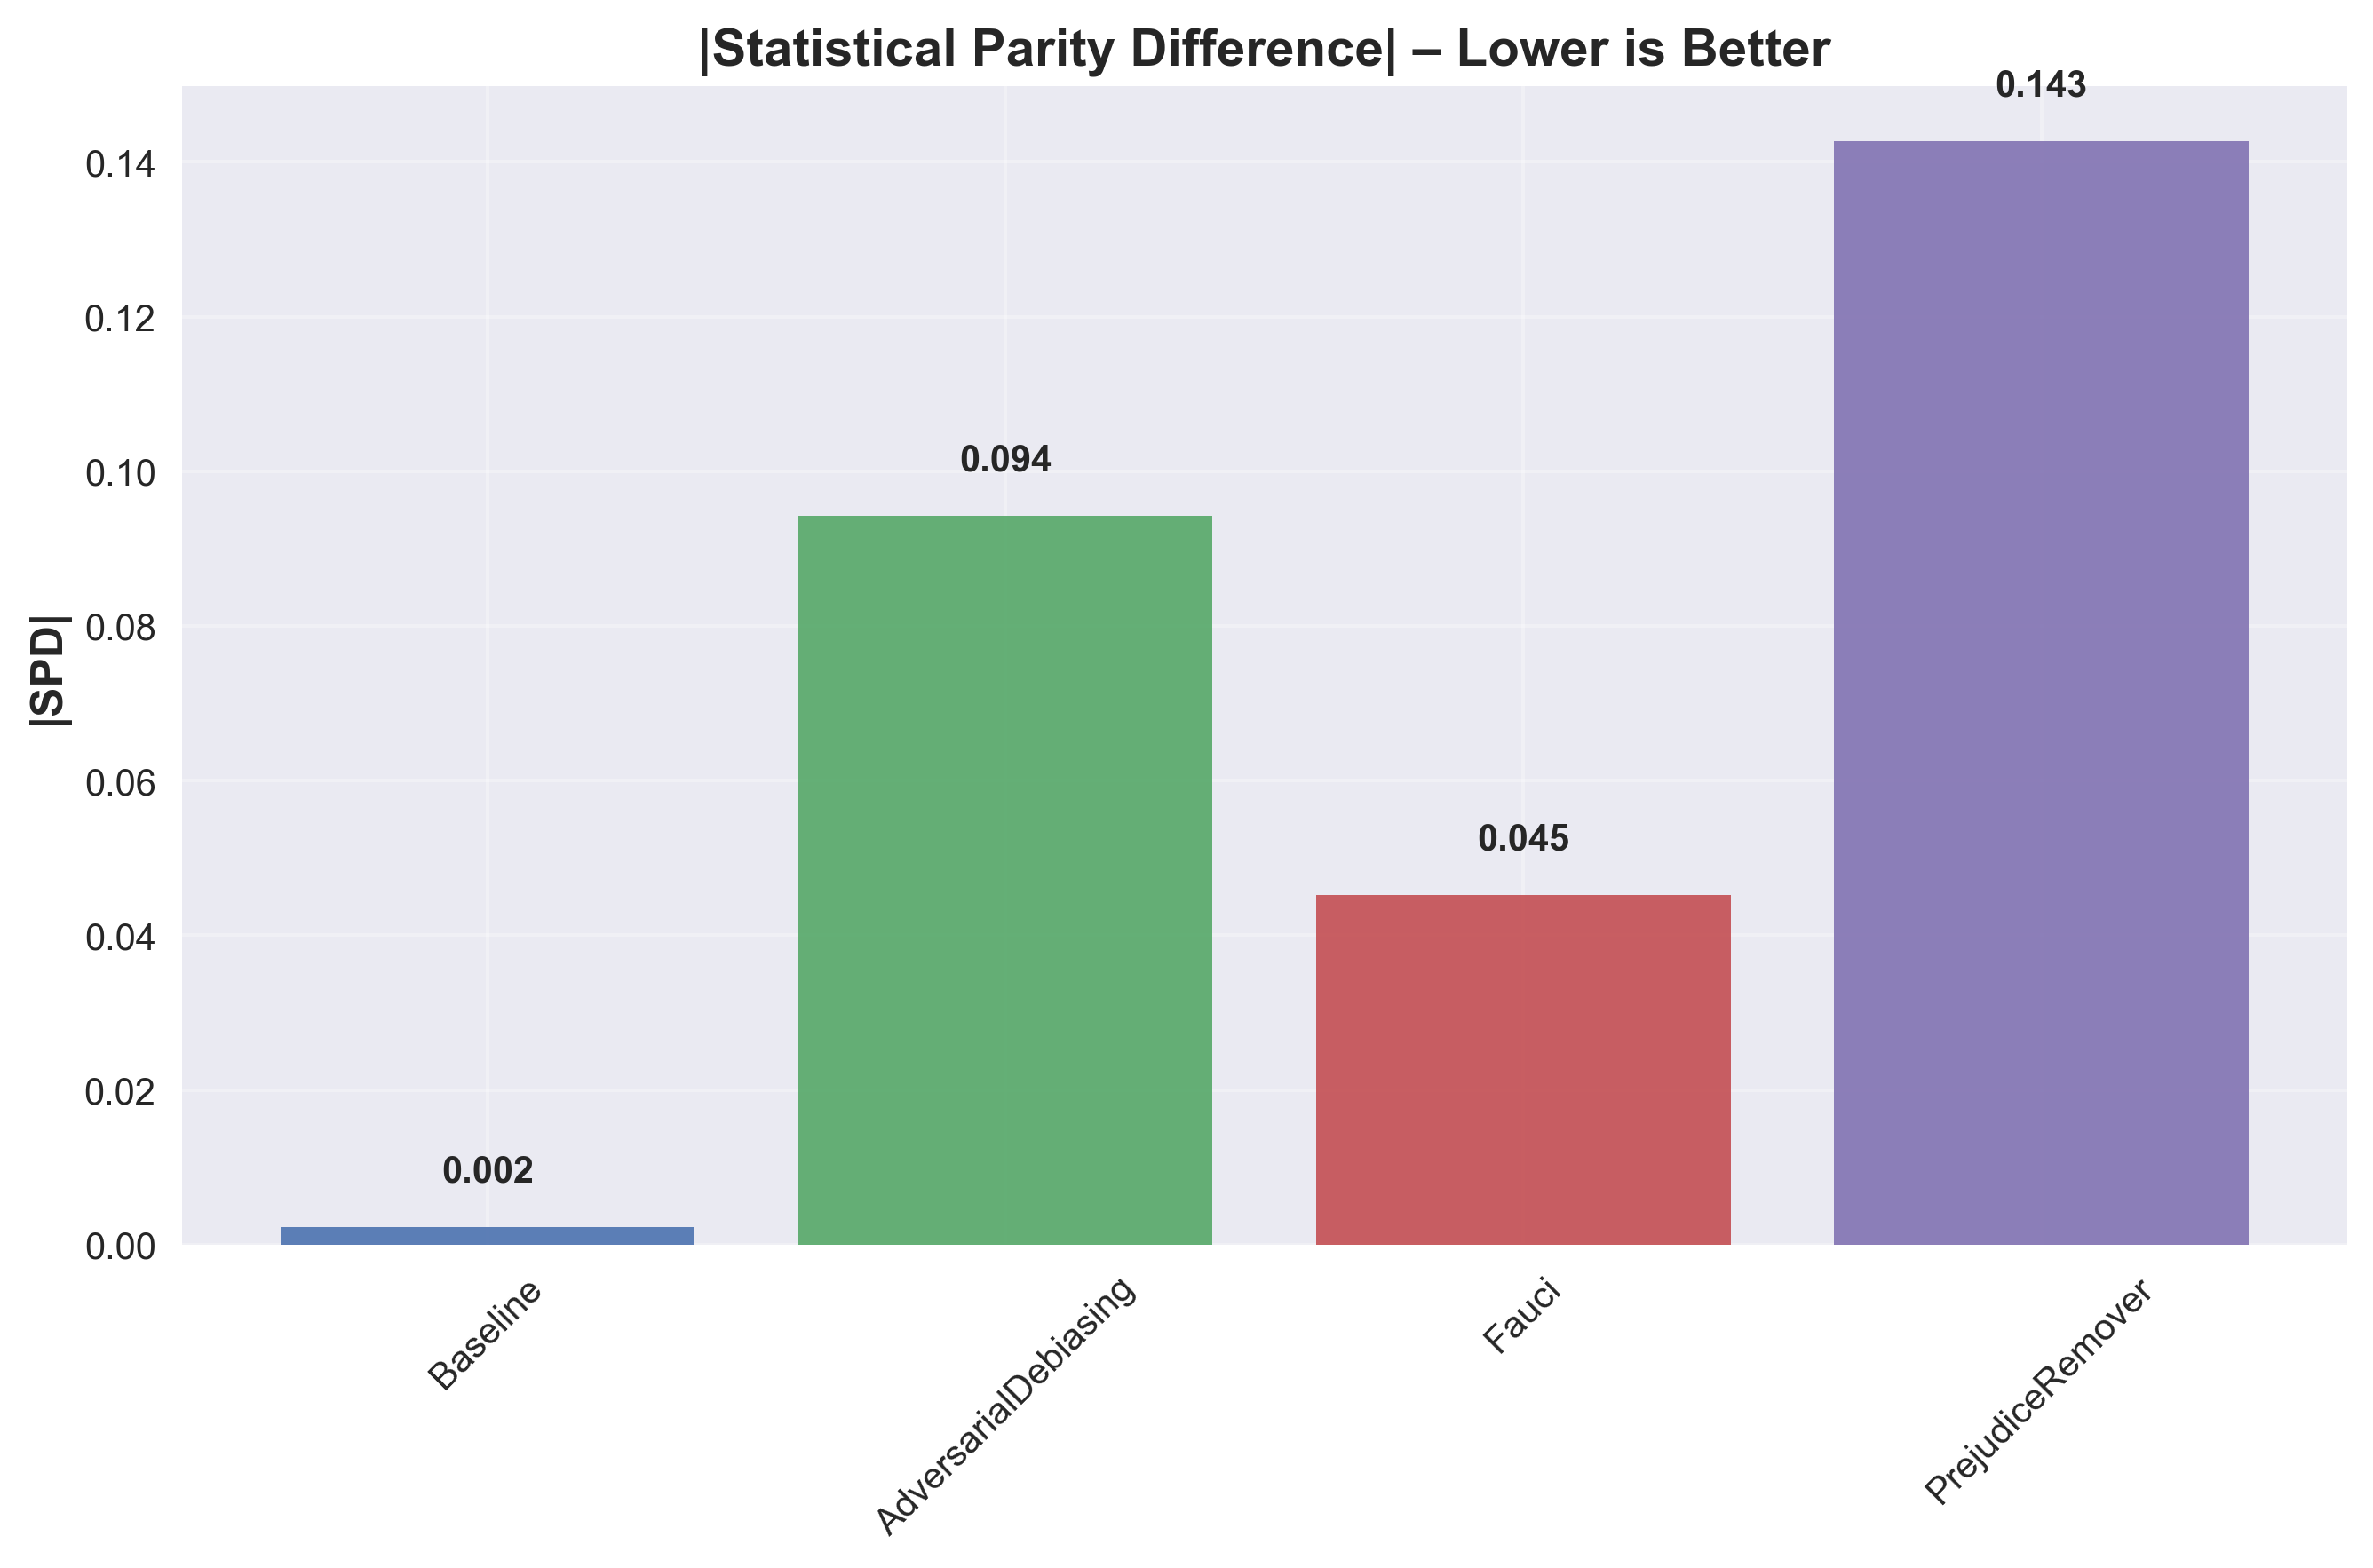
\includegraphics[width=\textwidth]{figures/inprocessing_results/inprocessing_spd_comparison.png}
    \caption{Statistical Parity Difference (SPD) for the baseline model and the models trained after applying in-processing algorithms. The SPD is computed on the test set of the Adult Income dataset.}
    \label{fig:inprocessing_results}
\end{figure}

\begin{figure}
    \centering
    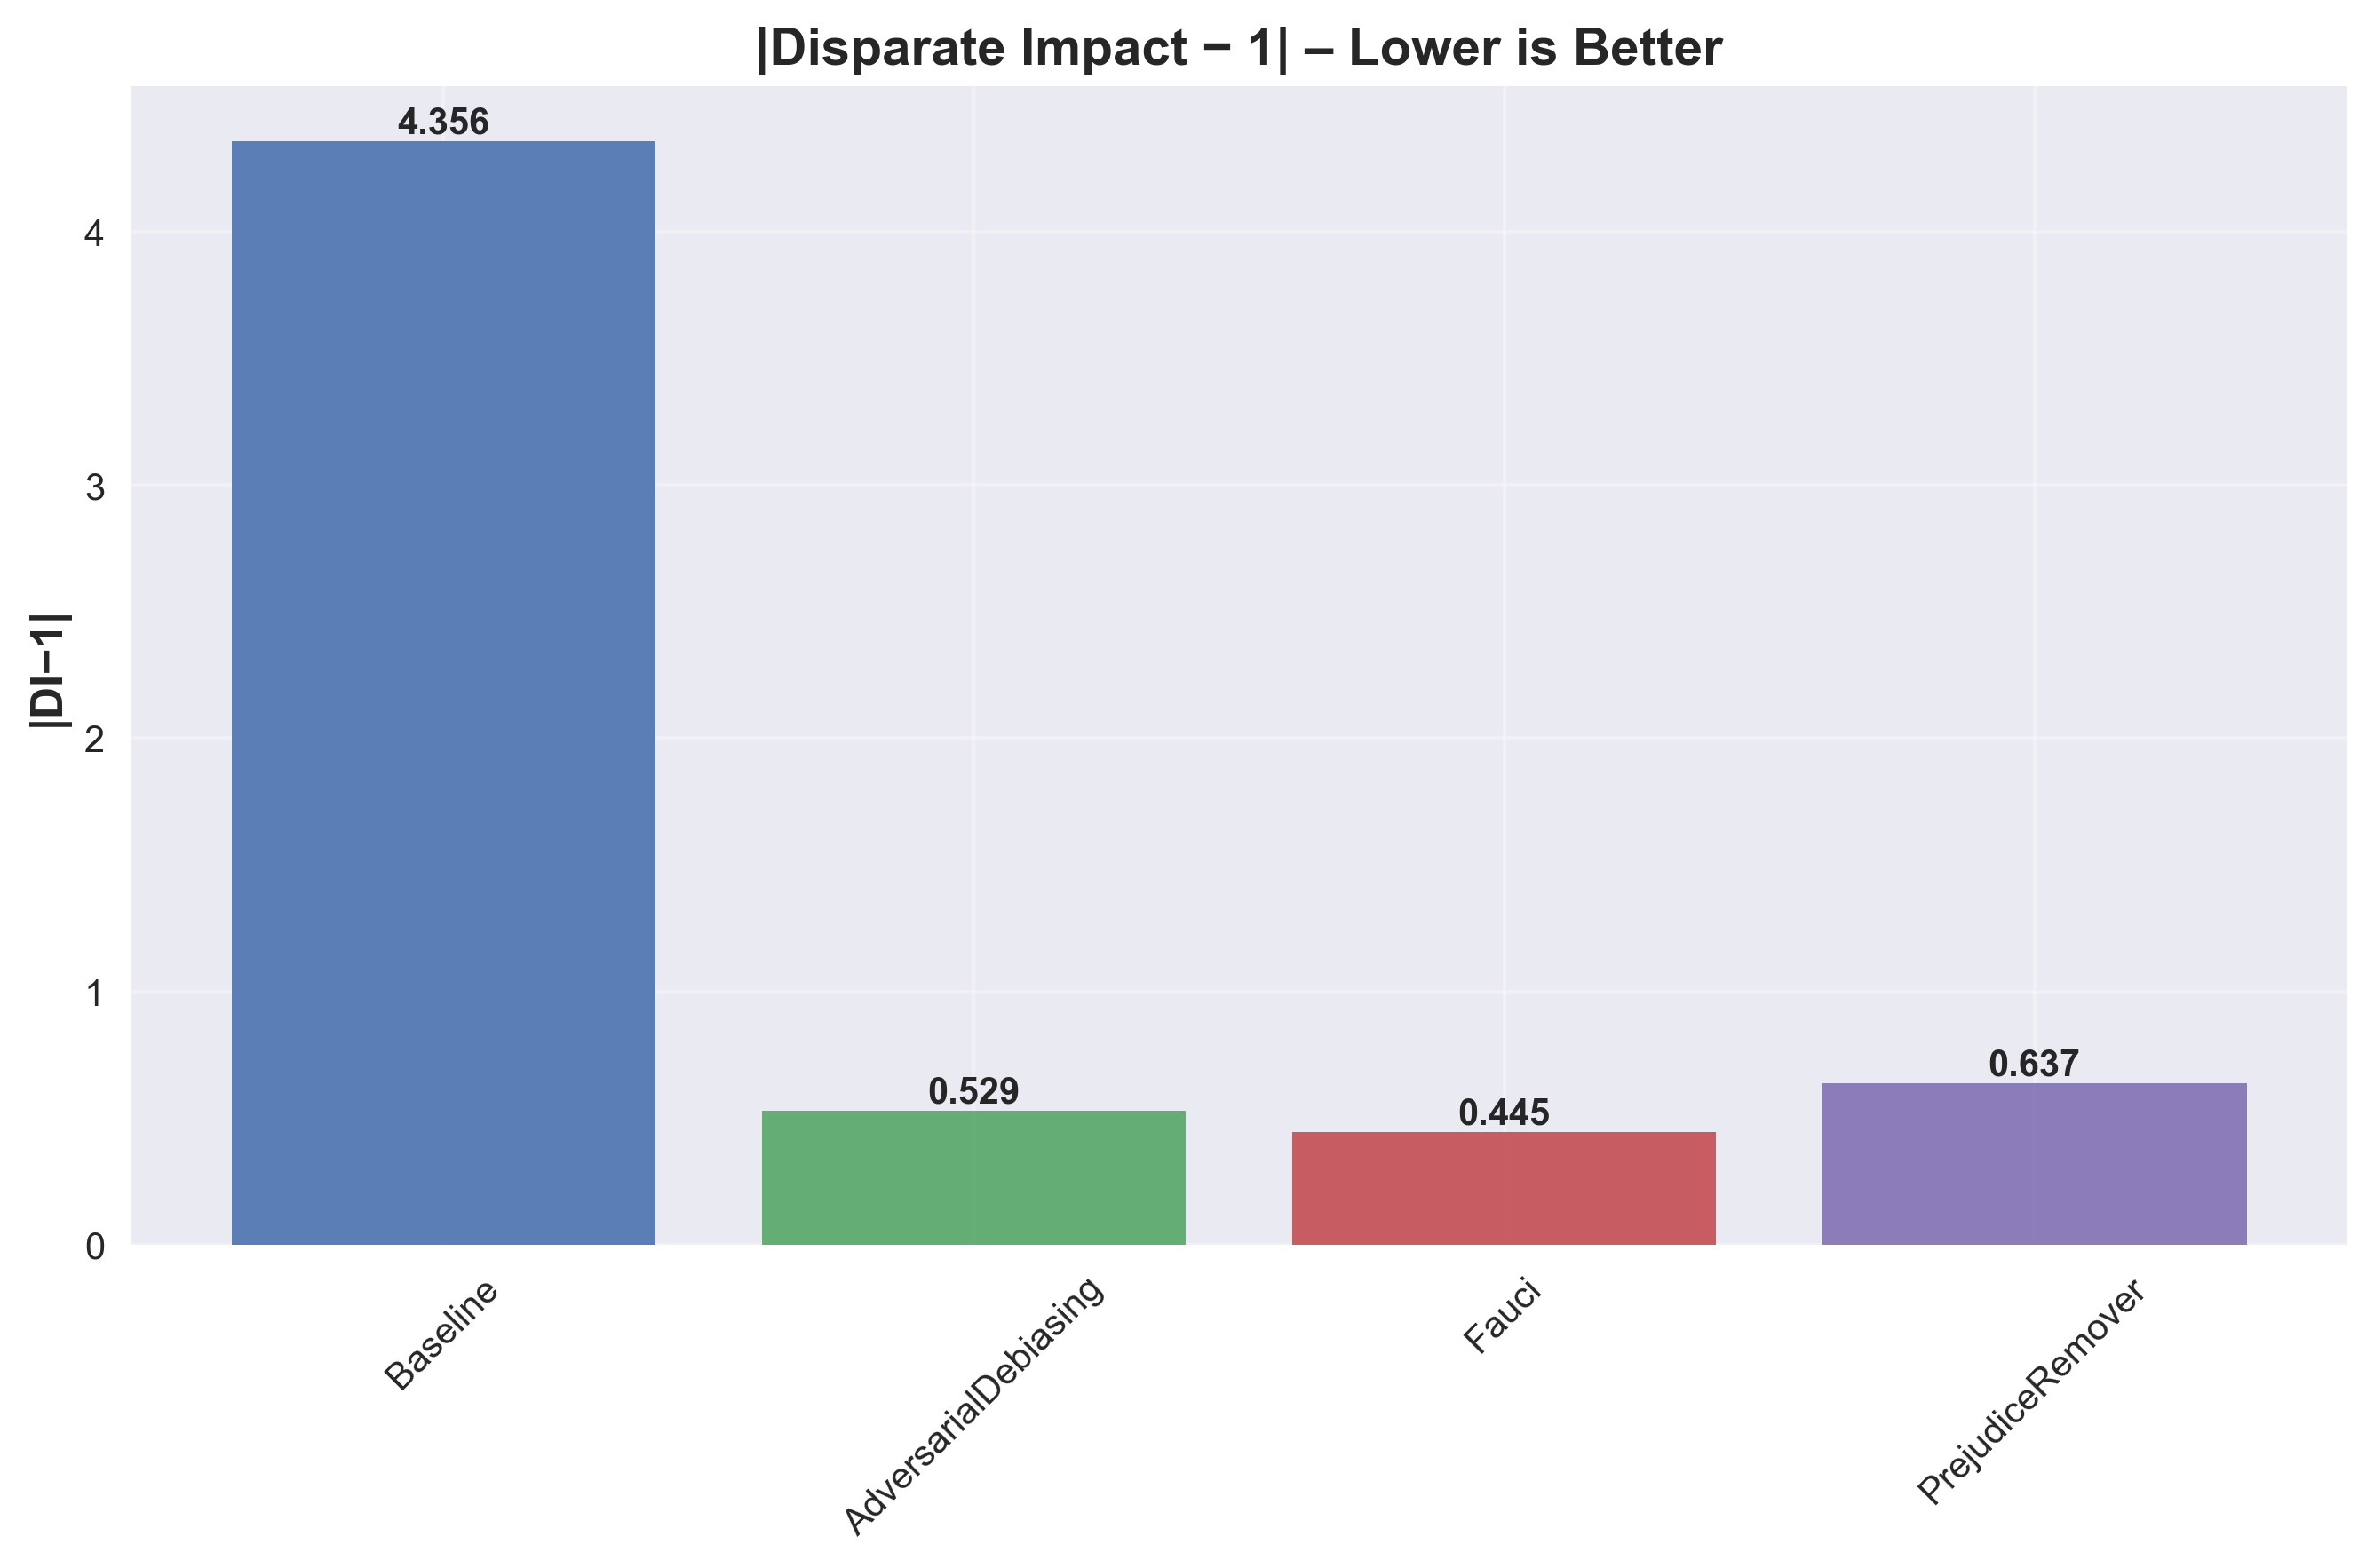
\includegraphics[width=\textwidth]{figures/inprocessing_results/inprocessing_di_comparison.png}
    \caption{Disparate Impact (DI) for the baseline model and the models trained after applying in-processing algorithms. The DI is computed on the test set of the Adult Income dataset.}
    \label{fig:inprocessing_results_di}
\end{figure}

From the results obtained by applying the algorithms in the in-processing module, we observe that all algorithms successfully reduce the Statistical Parity Difference (SPD) and Disparate Impact (DI) metrics compared to the baseline model. 

\subsection{Discussion}
The experimental results confirm that both the pre-processing and in-processing algorithms implemented in the fairness-aware library are effective in mitigating bias in classification tasks while preserving competitive predictive performance. Specifically, the Statistical Parity Difference (SPD) and Disparate Impact (DI) metrics exhibit substantial improvements over the baseline model, demonstrating a marked reduction in outcome disparities between sensitive groups.

In the in-processing experiments, the baseline classifier largely mirrors the class imbalance present in the training data: because roughly 75\% of the training instances belong to the negative class (label 0), the model predicts that outcome at a similar rate. In contrast, models trained with fairness constraints not only achieve a more balanced distribution of predicted classes — including a greater proportion of positive outcomes (accuracy) — but also exhibit improved fairness metrics. These results suggest that fairness-aware interventions can guide the learning process toward more equitable and accurate decision boundaries.


\chapter{Conclusion and Future Work}
This thesis introduced \textbf{FairLib}, a modular and extensible Python library specifically engineered to address the challenges of implementing fairness-aware machine learning in real-world scenarios. FairLib provides a unified, production-oriented interface that consolidates a broad spectrum of fairness metrics and bias mitigation algorithms, supporting both pre-processing and in-processing interventions. Its architecture is designed for seamless integration with popular machine learning frameworks such as scikit-learn and PyTorch, enabling practitioners to incorporate fairness considerations into their existing workflows with minimal friction.

The library’s design emphasizes usability, flexibility, and extensibility. By embedding metadata for sensitive attributes and targets directly into the data structure, FairLib streamlines the process of fairness evaluation and mitigation, reducing boilerplate and minimizing the risk of errors. The consistent API across all modules allows users to easily switch between different fairness metrics and mitigation strategies, facilitating rapid experimentation and comparative analysis. The inclusion of advanced algorithms—such as Reweighing, Learning Fair Representations, Disparate Impact Remover, Adversarial Debiasing, FaUCI, and Prejudice Remover—ensures that users can address a wide range of fairness definitions and application contexts.

Empirical evaluation on benchmark datasets, such as the Adult Income dataset, demonstrates that FairLib’s algorithms are effective in reducing bias as measured by key metrics like Statistical Parity Difference (SPD) and Disparate Impact (DI), while maintaining competitive predictive accuracy. The results confirm that both pre-processing and in-processing approaches implemented in FairLib can substantially mitigate unfairness in classification tasks, supporting more equitable model outcomes without prohibitive performance trade-offs.

Overall, FairLib advances the state of the art in fairness-aware machine learning tooling by lowering the barriers to adoption, promoting best practices, and enabling systematic, reproducible fairness interventions throughout the machine learning lifecycle. Its modular and extensible design positions it as a valuable resource for both researchers and practitioners seeking to build transparent, accountable, and equitable AI systems.

\section{Future Work}
A primary direction for future work is the addition of post-processing algorithms to FairLib. Post-processing techniques operate on the outputs of trained models, adjusting predictions to satisfy fairness constraints without requiring changes to the underlying data or model architecture. By supporting post-processing methods—such as Equalized Odds, Reject Option Classification, and Calibrated Equalized Odds—FairLib would enable practitioners to retrofit fairness guarantees onto existing models, even in scenarios where retraining is infeasible or access to sensitive attributes is restricted during training. Integrating these algorithms would further broaden the applicability of FairLib, allowing users to address fairness concerns at every stage of the machine learning pipeline and to comply with evolving regulatory requirements. Future releases will prioritize a unified interface for post-processing mitigations, ensuring consistency with the library’s existing pre-processing and in-processing modules.
In addition to post-processing, it is planned to expand the library's functionalities by including additional fairness metrics, new algorithms, and integration with other machine learning frameworks. It is also planned to improve the documentation and examples to facilitate adoption by a wider audience. Further empirical evaluations on different datasets and tasks are planned to validate the effectiveness of the library in real-world scenarios.



%----------------------------------------------------------------------------------------
% BIBLIOGRAPHY
%----------------------------------------------------------------------------------------

\backmatter

\nocite{*} % Remove this as soon as you have the first citation

\bibliographystyle{alpha}
\bibliography{bibliography}

\begin{acknowledgements} % this is optional

Un sentito grazie al \textbf{Prof.\ Giovanni Ciatto} per la disponibilità e i preziosi consigli che hanno arricchito il mio percorso accademico.  
Grazie per il clima accogliente nell’Area 4.0 e per tutto il supporto alla realizzazione di questo lavoro.
\\
Un ringraziamento speciale va alla \textbf{mia famiglia} per il loro sostegno incondizionato e per aver sempre creduto in me,  
supportandomi nei momenti di gioia e di difficoltà e appoggiando ogni mia scelta senza mai dubitare di me.
\\
\textbf{Margherita}, grazie di cuore per avermi sostenuto e, con infinita pazienza, sopportato in ogni momento; per esserti presa cura di me nei giorni più difficili e per aver esultato al mio fianco ad ogni traguardo.
\\
Grazie ai miei amici, compagni di viaggio e di avventure, che hanno condiviso con me gioie e difficoltà, rendendo ogni giornata più leggera.
\textit{In particolare:}
\\
\textbf{Giovanni Antonioni}
la tua precisione nei progetti, il sostegno costante e l’immancabile pizza patate e salsiccia sono stati pilastri di questo percorso. Grazie di cuore.
\\
\textbf{Luca Rubboli}
i tuoi consigli, i progetti condivisi e le grigliate in piscina hanno reso questi anni più leggeri. Grazie! Chissà se saprò mai che sapore ha un caffè offerto da te\dots
\\
\textbf{Francesco Magnani}
il tuo aiuto nello studio e nei progetti, insieme ai mille giochi da tavolo, si è rivelato preziosissimo in questi ultimi anni. Grazie di avermi fatto scoprire Outer Wilds!
\\
\textbf{Matteo Belletti}
grazie per il tuo supporto e per i nostri splendidi discorsi sulla vita e sul futuro; spero che, prima o poi, tu ti riprenda dall’essere «cotto duro».
\\
\textbf{Tirso Buttafuoco}
anche a chilometri di distanza, non è mai mancata una tua parola di conforto. Grazie per il sostegno e per il tuo instancabile tentativo di battermi a Yu-Gi-Oh!: continua a provare, magari un giorno ci riuscirai.



\end{acknowledgements}

\end{document}
